\documentclass[10pt, a4paper]{article}
\usepackage{subfigure,layout, amssymb, graphicx, textcomp, url, color}
\newcommand{\comment}[1]{} % en kommentar.
\newcommand{\partners}{\emph{Partners:~}}
\newcommand{\period}{\emph{Period:~}}
\newcommand{\aabstract}[1]{\emph{Abstract:~}#1}
\newcommand{\aauthor}[1]{\emph{Author:~}#1\\}
\newcommand{\aauthors}[1]{\emph{Authors:~}#1\\}
\newcommand{\bbook}[1]{\emph{Book:}~#1\\}
\newcommand{\ccomment}[1]{\emph{Comment:~}#1\\}
\newcommand{\cconference}[1]{\emph{Conference:~}#1}
\newcommand{\eeditor}[1]{\emph{Editor:~}#1\\}
\newcommand{\eeditors}[1]{\emph{Editors:~}#1\\}
\newcommand{\ffunding}[1]{\emph{Funding:~}#1\\}
\newcommand{\jjournal}[1]{\emph{Journal:~}#1\\}
\newcommand{\ppartner}[1]{\emph{Partner:~}#1\\}
\newcommand{\ppartners}[1]{\emph{Partners:~}#1\\}
\newcommand{\ppublisher}[1]{\emph{Publisher:~}#1}
\newcommand{\pperiod}[1]{\emph{Period:~}#1\\}
\newcommand{\ttitle}[1]{\item \textbf{#1}\\}
\newcommand{\cba}{CBA}
\newcommand{\uu}{UU}

\begin{document}

\newcommand{\commentfigure}[1]{}
\newcommand{\researcharea}[1]{\subsection{#1}}

\section{Research}\label{research}
\label{research_proj}
{\large
Our research activities are conducted in a large number of projects, both very application oriented and theoretical, both large and small, both long-running and short. Our largest application field is biomedicine, with many projects developing methods for analysing microscopic images of molecules, viruses, cells, and tissue. In addition we also have much going on in analysis and visualization of 3D medical images. In the latter case we develop haptic tools for interactive exploration of such images. We are also active in the analysis of wood and wood fibre based materials. In addition to these areas especially mentioned in our charter we are involved in other applications, the biggest of which is analysis of old, handwritten texts. There are also projects for the urban and rural environments -- and for tracking bees. In our application projects we have a partner with a set of images and a problem getting information from them, a problem interesting enough to generate new analysis methods. We also develop new, general theory for image analysis and visualization, especially in digital geometry and mathematical morphology and usually in volume images, but not as much as we would like to. The reason is that it is much easier to get grants for applications of image analysis than for image analysis itself.

In Section ~\ref{partners} we have collected all partners, national and international, with which we had active co-operation in 2013. They can all also be found somewhere else in this report.}
\vfill
\subsection{Forestry related applications}
\begin{enumerate}
\setcounter{enumi}{0}

%--------------------------------------------------------------

\item
\textbf{Diffraction Artifact Reduction in \textmu CT Imaging}\\
Erik Wernersson, Cris Luengo, Anders Brun, Gunilla Borgefors \\
\ppartners{Jan Van den Bulcke, Dept.~of Forest and Water Management, Ghent University, Belgium; Matthieu Boone, Dept.~of Physics and Astronomy, Ghent University, Belgium}
\ffunding{S-faculty, SLU}
\pperiod{1009 --}
\aabstract{When imaging wood based materials, diffraction causes artifacts especially around sharp edges. While sometimes useful, and the only
measurable properties of the imaged objects, they might as well be a nuisance which hinders proper analysis of the absorption coefficient.
In this project, different ways to reduce such artifacts are investigated, especially in already reconstructed images. Compare to previous approaches, this is much faster and does not require that the original projection images are stored.  For an example of the artifact, see Fig.~\ref{fig:diffraction}.

We have had one article published in Journal of the Optical Society of America during 2013. One of the main results is that it is at least as good to remove the diffraction artifacts after the reconstruction as before it.}

\begin{figure}[!htbp]
\subfigure[]{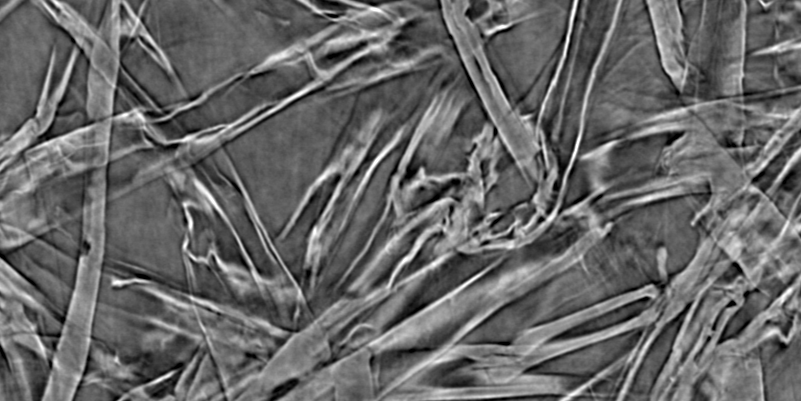
\includegraphics[width=0.495\textwidth]{figures/research/org.png}}
\hfill
\subfigure[]{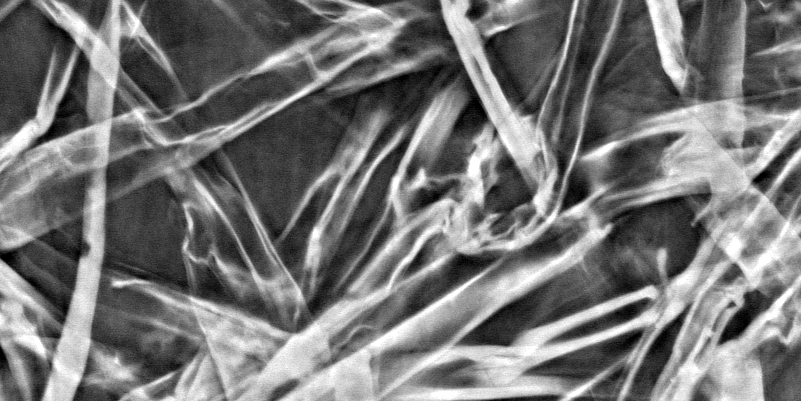
\includegraphics[width=0.495\textwidth]{figures/research/filt.png}}
\caption{\label{fig:diffraction} A slice from a volume image of a paper sample. (a) directly reconstructed, a mixed imaged with both phase and amplitude. (b) phase contribution removed to reveal the amplitude or absorption.}
\end{figure}

%--------------------------------------------------------------

\item 
\label{proj:paper}
\textbf{Image Analysis of the Internal Structure of Paper and Wood Fibre Based Composite Materials in 3D~images}\\% \textcolor{red}{To Be Removed If No Updates}}\\
Erik Wernersson, Anders Brun, Cris Luengo, Gunilla Borgefors\\
\ppartners{Gary Chinga, Norwegian Pulp and Fibre Research Institute, Trondheim, Norway;
Catherine \"{O}stlund, Innventia, Stockholm; Thomas Joffre, Dept.~of Engineering Sciences, Applied
Mechanics, UU; Arttu Miettinen, Dept.~of Physics, University of Jyv\"{a}skyl\"{a} (UJ), Finland;  Joakim Lindblad, University of Novi Sad, Serbia; Svetlana Borodulina, Department of Solid Mechanics and BiMaC Innovation Center, KTH
}
\ffunding{S-faculty, SLU; WoodWisdom-Net}
\pperiod{0406--}
\newpage
\aabstract{The internal structure of paper is important because many of its properties correspond directly to the properties of single
fibres and their interaction in the fibre network. How single fibres in paper bond and how this affects paper quality is not fully
understood, since most structure analysis of paper has been performed in cross-sectional, two-dimensional (2D) images whereas paper is a
complex, three-dimensional (3D) structure.

Another application for wood fibres that has recently gained interest is wood polymer composite materials. The properties of these materials
do not only depend on the structure of the fibre network, but also on the interaction between the fibres and the polymer matrix surrounding
the fibres.

Advances in imaging technology have made it possible to acquire 3D images of paper and wood polymer composite materials. In this project,
image analysis methods for characterizing the 3D material structure in such images are developed. The detailed knowledge of the material
structure attainable with these methods is useful for improving material properties and for developing new materials.

The project objective is to achieve a complete segmentation of individual fibres and pores in volume images of the material. Given such a segmentation, any desired measurement of the internal structure is available. Measurements on individual fibres and the structural
arrangement of fibres can then be related to macroscopic material properties.

In this project, different volume images of paper and composite materials are available: one volume created from a series of 2D scanning electron microscopy (SEM) images at StoraEnso, Falun; and X-ray microtomography volume images of paper and composite samples imaged at the European Synchrotron Radiation Facility (ESRF) in Grenoble, France, at the Paul Scherrer Institut (PSI) in Villigen, Switzerland and also from tabletop scanners at University of Jyv\"askyl\"a, Finland, UU, and Innventia, Stockholm.}

%----------------------------------------------------------------------------------------------------------------------------------------------

\item \label{proj:woodSynth}
\textbf{Generation of Synthetic \textmu CT Volumes}\\ %\textcolor{red}{To Be Removed If No Updates}}\\
Erik Wernersson, Cris Luengo, Anders Brun, Catherine \"{O}stlund, Gunilla Borgefors \\
\ppartners{Norwegian Pulp and Paper Research Institute (PFI), Trondheim, Norway; Innventia, Stockholm; Dept.~of Engineering Sciences, Applied Mechanics, \uu; Dept.~of Physics, University of Jyv\"{a}skyl\"{a} (UJ), Finland; SINTEF Materials and Chemistry, Norway; Ris{\o} National Laboratory, Technical University of Denmark}
\ffunding{S-faculty, SLU; WoodWisdom-Net}
\pperiod{0901--}
\newpage
\aabstract{It is of great importance to evaluate the performance and stability of new methods. It is often hard to do so, when working with natural materials, since no true answer is available. With this project we aim to create highly realistic reference images that can be used to
evaluate new and existing methods designed for characterisation of fibrous materials from \textmu CT.

Within the project, methods have been developed to generate and pack synthetic wood fibres as well as to simulate \textmu CT acquisition
systems with characteristic artifacts.}

%----------------------------------------------------------------------------------------------------------------------------------------------

\item
\textbf{Ring Width and Density Profiling with Helical CT}\\
Erik Wernersson, Cris Luengo, Anders Brun, Gunilla Borgefors \\
\ppartners{Jan Van den Bulcke, Dept.~of Forest and Water Management, Ghent University, Belgium}
\ffunding{S-faculty, SLU}
\pperiod{1201 --}
\aabstract{Dendrochronology relies on accurate measurements of annual ring widths. The most common method is to use a flatbed scanner to
acquire high resolution images of polished wood surfaces. In this project we investigate potential gains using a helical xray device
which produces volume images. Direct advantages include non destructive and simplified sample preparation procedures as well as compensation for the orientation of the inner structure which can not be seen with ordinary flatbed scans. It is also possible to find density profiles using the same images. During 2013, one article was submitted to Dendrochronologia which will be published during 2014.}

\clearpage

%----------------------------------------------------------------------------------------------------------------------------------------------
%----------------------------------------------------------------------------------------------------------------------------------------------
%----------------------------------------------------------------------------------------------------------------------------------------------
%----------------------------------------------------------------------------------------------------------------------------------------------
%----------------------------------------------------------------------------------------------------------------------------------------------

\subsection{Analysis of microscopic biomedical images}

% AAA

\item
\textbf{Identification of Highly Pathogenic Viruses in Transmission Electron Microscopy Images} \label{proj:PVS2}
Gustaf Kylberg, Ida-Maria Sintorn, Ewert Bengtsson, Gunilla Borgefors\\
\ppartner{Vironova AB; Delong Instruments, Brno, Czech Republic; Ali Mirazimi, Kjell-Olof H\"{o}glund, Centre for Microbiological Preparedness; Swedish Institute for Infectious Disease Control (SMI)}
\ffunding{Swedish Civil Contingencies Agency (MSB); Swedish Defense Materiel Administration (FMV); Swedish Agency for Innovative Systems (VINNOVA). Eurostar project E!6143}
\pperiod{0801--}
\aabstract{This project aims at automating the virus identification process in high resolution TEM images. This, in combination with Project \ref{proj:PVS1} create a rapid, objective, and user independent virus diagnostic system. The identification task consists of method development for segmenting virus particles with different shapes and sizes and extracting descriptive features of both shape and texture to enable the classification into virus species. Texture features such as variants of Local Binary Patterns and Regional Moments (filter banks constructed from orthogonal moments), are being evaluated on virus textures as well as other texture datasets to get a deeper understanding of the discriminant power of the features under different conditions. A paper evaluating the discriminating power and noise robustness for Local Binary Pattern variants was published during 2013, and a poster about the project was presented at the Microscopy Conference in Regensburg, Germany in August.} 

% BBB

\item
\textbf{The miniTEM Project - Development of a Desk-top TEM with Automated Image Acquisition}\\ \label{proj:PVS1}
Gustaf Kylberg, Ida-Maria Sintorn, Ewert Bengtsson, Gunilla Borgefors\\
\ppartner{Vironova AB; Delong Instruments, Brno, Czech Republic}
\ffunding{Eurostar project E!6143}
\pperiod{1107--}
\aabstract{Transmission electron microscopy (TEM) is an important clinical diagnostic and material analysis tool. Transmission electron microscopes are expensive, complex, sensitive and bulky machines, often housed in specially built rooms to avoid vibrations affecting the imaging process. They are to a very large extent manually operated, meaning that an expert in electron microscopy and preferably also in the  application at hand needs to perform the analysis at the microscope, an often very time consuming task. 
 
This project aims at developing the miniTEM, shown in Figure~\ref{fig:miniTEM}(left), a desk-top low voltage TEM designed for imaging biological samples, with a high degree of automation regarding instrument alignment, image acquisition and analysis. The goal is a small, cheap, robust, and easy to use system that requires no more training than any simple lab equipment, and can be hosted in any office or lab (even mobile).

Automating the image acquisition process is key for reducing the manual input and making the imaging and analysis more objective. A few different options for automated image acquisition are being developed and will be incorporated in the instrument. The first is acquisition of images at random positions on the grid. The second is to search for a specific structure/object and only acquire (store) the images containing the structure/object of interest. The third is similar to the second approach but embedded in a multi-scale approach with the goal to make the acquisition more efficient.

The very first images from the miniTEM were acquired at the end of 2013. An example image of nanotubes with an approximate thickness of 15nm are shown in Figure~\ref{fig:miniTEM}(right). Work on optimizing the sample preparation procedure for improved electron transmittance was presented at the Microscopy Conference in Regensburg, Germany in August.}

\begin{figure*}[!h]
\centering
\subfigure[]{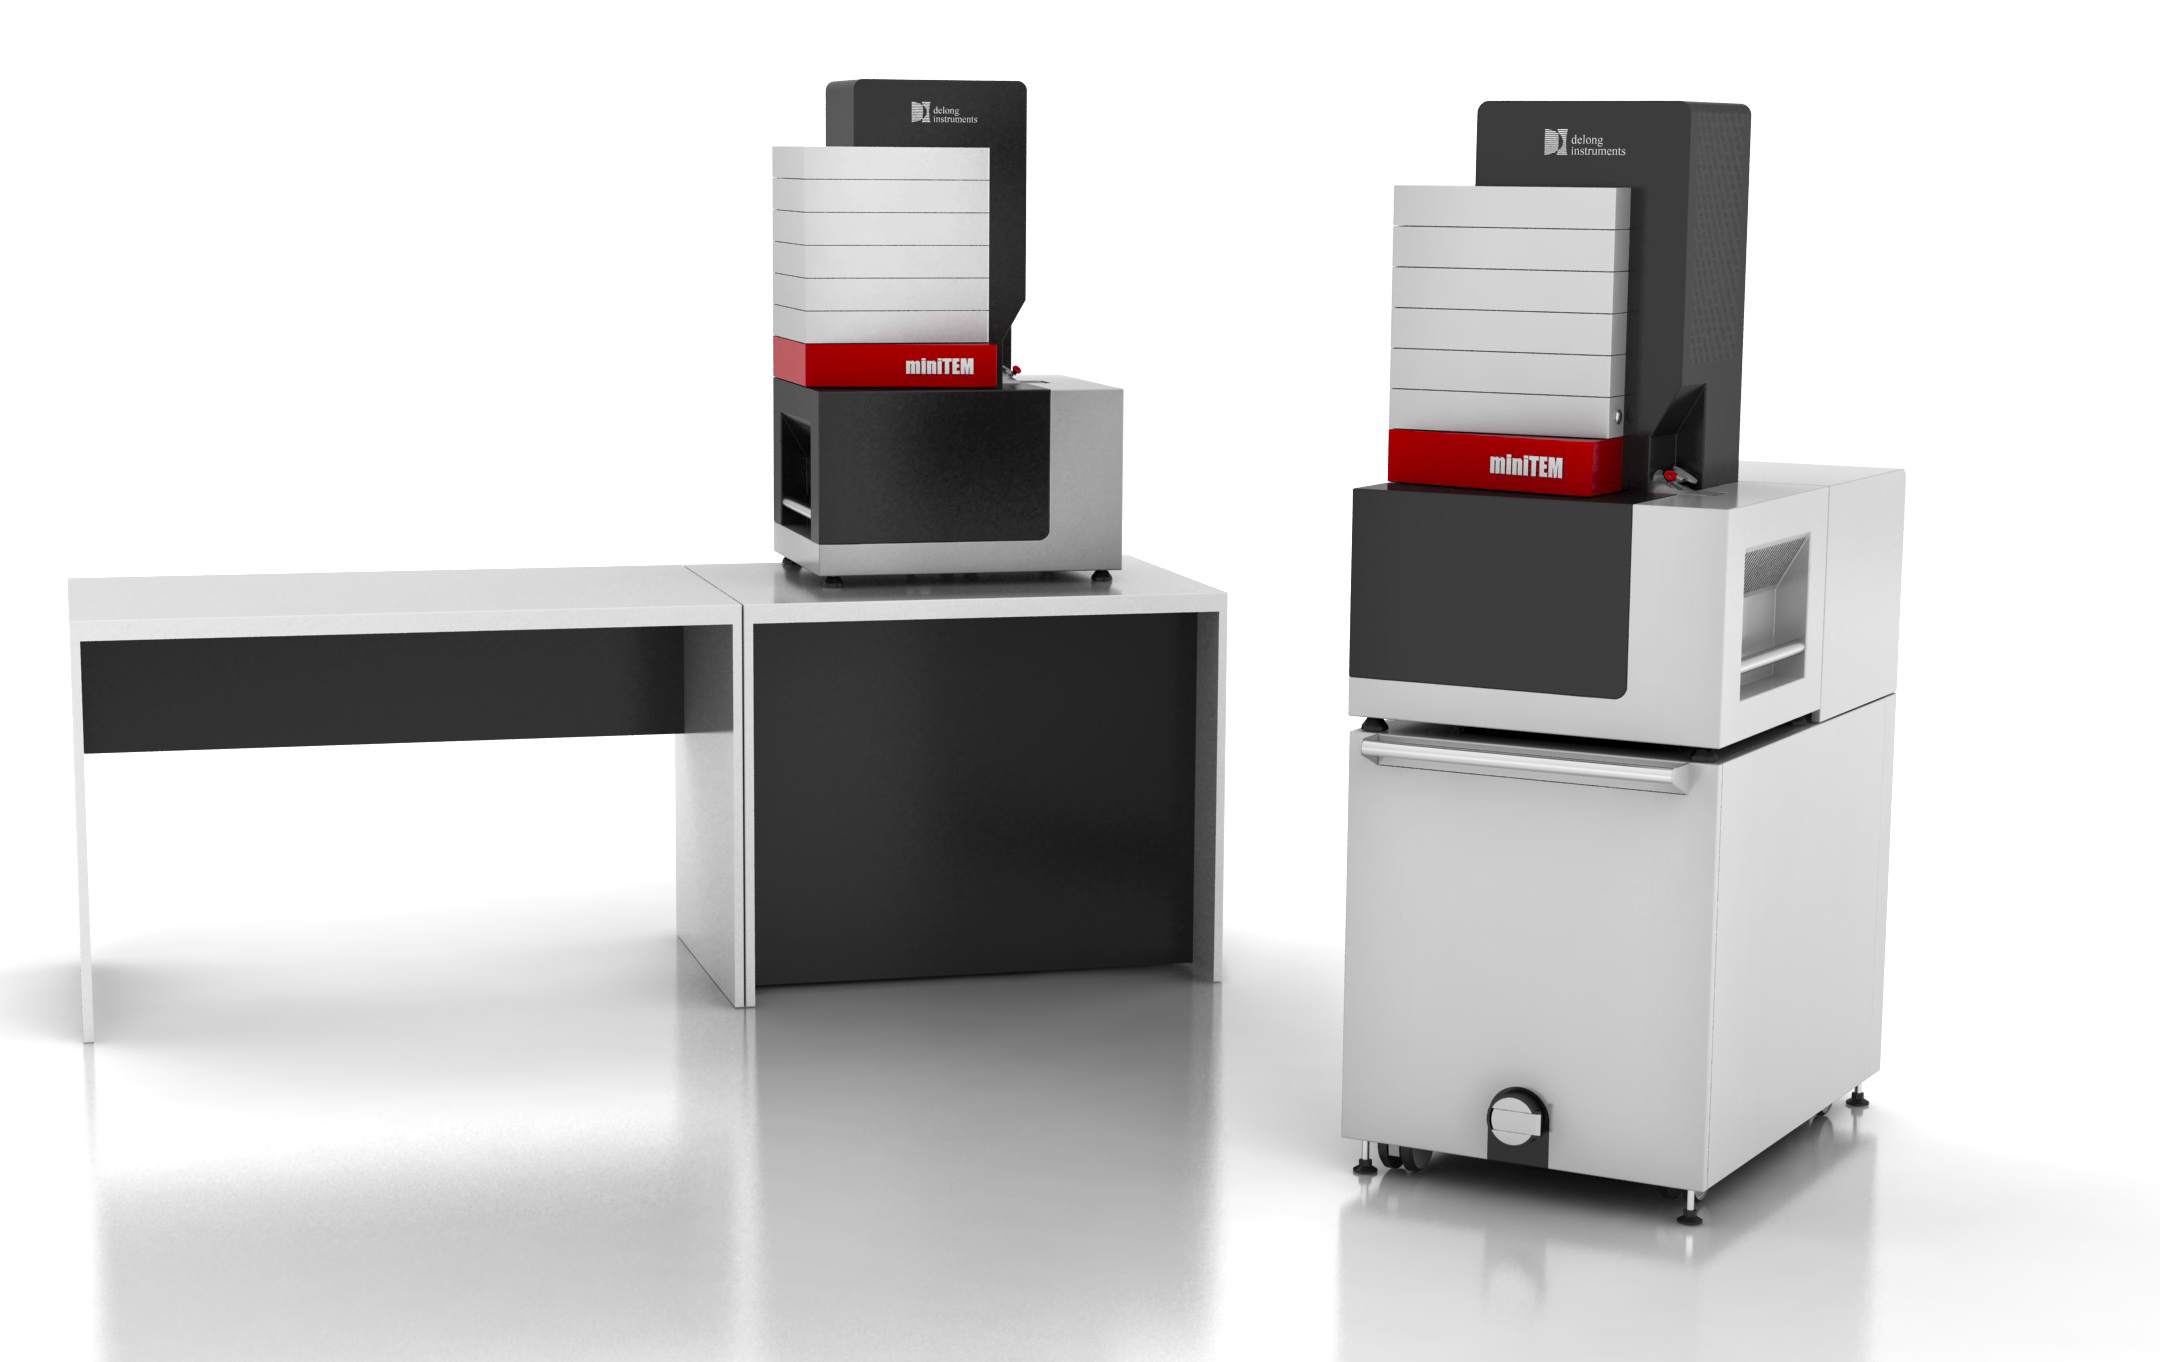
\includegraphics[width=0.36\linewidth]{figures/research/miniTEMLarge.png}}
\subfigure[]{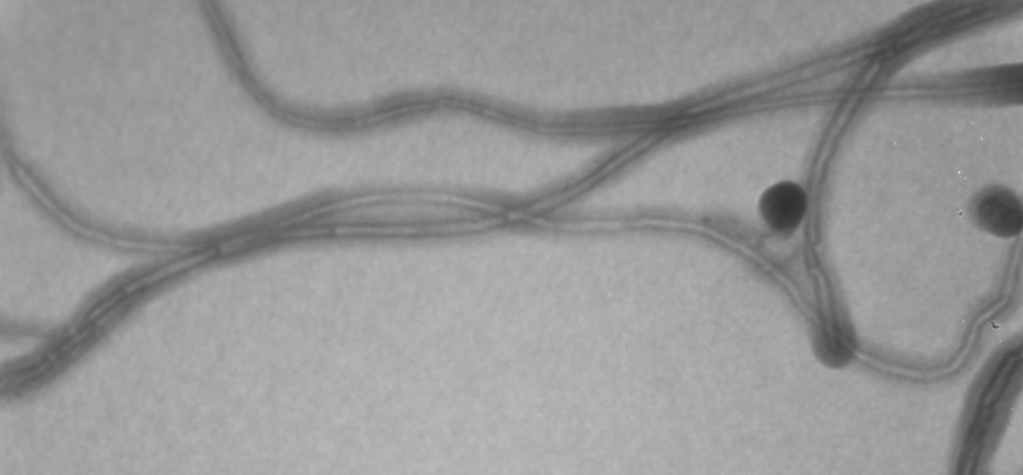
\includegraphics[width=0.48\linewidth]{figures/research/miniTEMnanotubulescutwider.png}}
\caption{Desk-top and mobile version of the miniTEM (left). Nanotubes, approximately 15nm thick, the first image acquired with the miniTEM (right).}
\label{fig:miniTEM}
\end{figure*}

% CCC
\vspace*{-2mm}
\item 
\textbf{Detection and Localization of Florescent Signals in STORM Data Using Compressed Sensing}\\
Omer Ishaq, Alexandra Pacureanu, Carolina W\"{a}hlby\\
\ppartners{Johan Elf, Gustaf Ullman, Fredrik Persson, Dept.~of Cell \& Molecular Biology, UU}
\ffunding{SciLifeLab Uppsala, eSSENCE, VR junior researcher grant to CW}
\pperiod{1211-}
\aabstract{Stochastic optical reconstruction microscopy (STORM) is a super-resolution microscopy image acquisition technique for single-molecule localization. Like other stochastic super-resolution microscopy techniques it incorporates a trade-off between spatial- and temporal-resolution. Recently, a compressed-sensing (CS) based variant of STORM, called FasterSTORM, has been developed which substantially increases the temporal sampling of a stack of STORM image frames. This improvement is realized by increasing the density of activated fluorophores in each frame, followed by a subsequent CS-based retrieval of single-molecule positions even with overlapping fluorescent signals.  However, the CS-based retrieval/decoding step is time consuming and can take as much as three hours for each image frame. We have accelerated the FasterSTORM method through parallel processing on multi-core processors. Additionally, we have tested and tried a number of L\raisebox{-.4ex}{\scriptsize 1}-solvers for CS-based recovery of molecule positions. A paper comparing convex and greedy solvers and evaluating the sensitivity of the FasterSTORM to estimation bias of the point spread function (PSF) was submitted to a conference. We are in the process of comparing the performance of the Faster STORM against a wavelet-based approach to localize fluorescent signals in time-lapse images of bacterial cells.}

%DDD

\item 
\textbf{\emph{In Situ} Sequencing of mRNA}\\
Carolina W\"{a}hlby, Alexandra Pacureanu, Petter Ranefall \\
\ppartners{Mats Nilsson, Rongqin Ke, Marco Mignardi, Thomas Hauling, SciLifeLab Stockholm}
\ffunding{SciLifeLab Uppsala; TN-faculty, UU}
\pperiod{1109--}
\aabstract{Profiling of gene expression is prerequisite for understanding the function of cells, organs and organisms, in health and disease. The sequencing techniques currently in use rely on homogenization of the samples. Therefore, the obtained information represents either the average expression profile of the tissue sample or expression profiles of isolated single cells. Our collaborators have developed a new molecular method, enabling \emph{in situ} sequencing of mRNA, so that protein expression can be observed directly in cultured cells or tissue samples. We have developed image analysis tools for automated analysis of sequencing data, mapping, and visualization of gene expression patterns (Fig. \ref{fig:carolina_insitu}). In 2013 we published a paper in Nature Methods and a conference paper focusing on the image analysis was accepted for publication in proceedings of the IEEE International Symposium on Biomedical Imaging (ISBI), Beijing 2014.}

\begin{figure}[!tb]
\centering
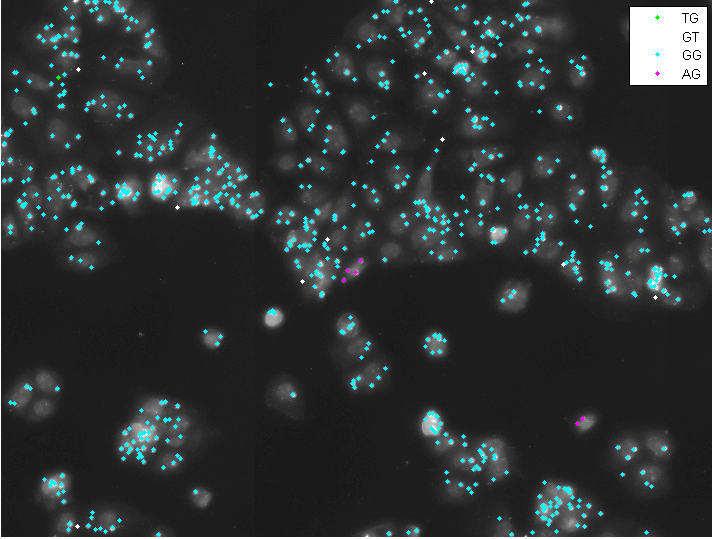
\includegraphics[width=0.56\textwidth]{figures/research/insitu.png}
\caption{\label{fig:carolina_insitu} Demonstrating the sensitivity of the sequencing method (finding rare mutants) - cell culture of ONCO-DG1 with wild type KRAS (GG) spiked with A549 cells (1:100) with mutant KRAS (AG). Note how the majority of the cells express the wild type gene (cyan), while a few express multiple copies of the mutated gene (pink).} 
\end{figure}

% EEE

\item 
\textbf{Evaluation of the Effect of Compaction Oligonucleotides on the Strength and Integrity of Florescent Signals }\\
Omer Ishaq, Petter Ranefall, Carolina W\"{a}hlby\\
\ppartners{Carl-Magnus Clausson, Linda Andersson, Ola S\"{o}derberg, Dept.~of Immunology, Genetics and Pathology}
\ffunding{SciLife Lab Uppsala}
\pperiod{1310--}
\aabstract{Rolling circle amplification (RCA) performs nucleic acid replication for rapid synthesis of multiple concatenated copies of circular DNA. These molecules can be visually observed through the use of florescent markers. Moreover, the introduction of a compaction oligonucleotide during RCA results in brighter and more compact signals. The project aims to evaluate the effect of compaction oligonucleotides on the strength and integrity of florescent signals.}





\item 
\textbf{Skeleton-Based Vascular Segmentation at Interactive Speed} \\
Krist\'{i}na Lidayov\'{a}, Hans Frimmel, Ewert Bengtsson \\
\ppartner{ \"{O}rjan Smedby, Chunliang Wang, Center for Medical Image Science and Visualization (CMIV), Link\"{o}ping University}
\ffunding{VR grant to \"{O}rjan Smedby}
\pperiod{1207--}
\aabstract{Precise segmentation of vascular structures is crucial for studying the effect of stenoses on arterial blood flow. The goal of this project is to develop and evaluate vascular segmentation, which will be fast enough to permit interactive clinical use. The first part is the extraction of the centerline tree (skeleton) from the gray-scale CT image. Later this skeleton is used as a seed region (Figure \ref{fig:Skeleton}). The method should offer sub-voxel accuracy.

During the last year we improved the software for fast vessel centerline tree extraction. The method has been tested on several CT datasets and the results look promissing. Generally all main vessel centerlines are detected, but some improvement  needs to be done in order to remove some false positive centerlines.}

\begin{figure}[!htbp]
\centering
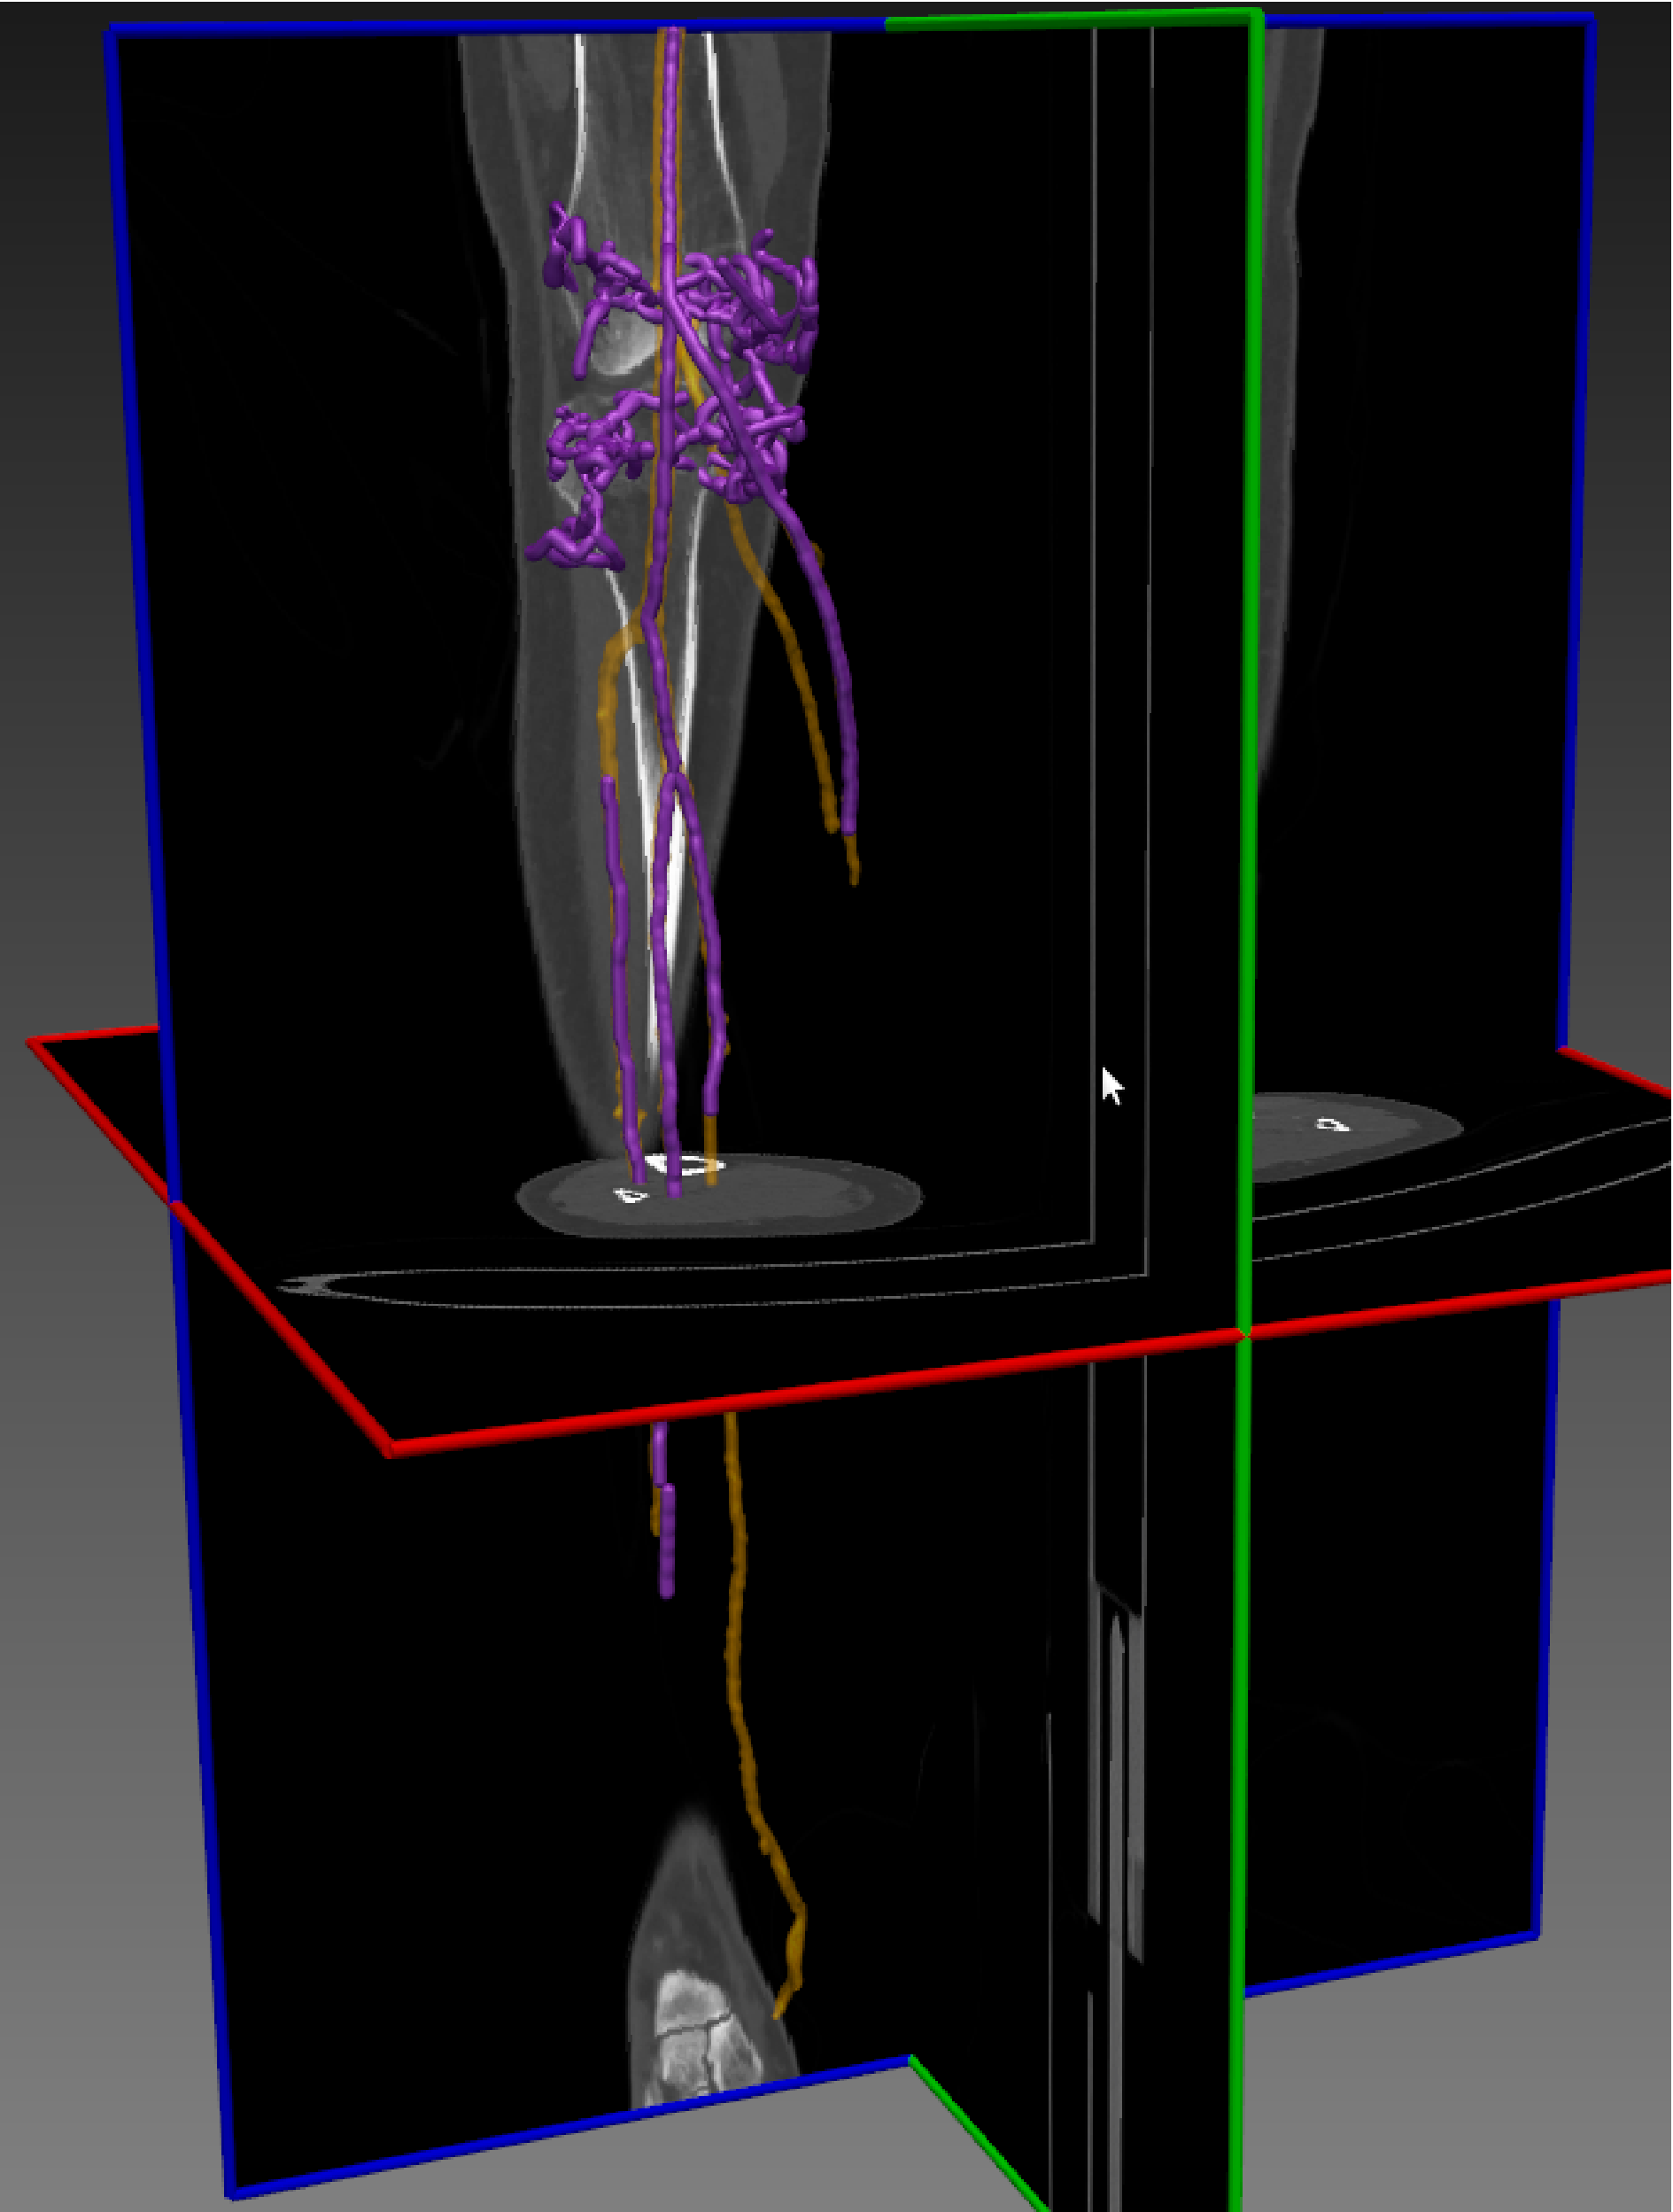
\includegraphics[width=85mm,height=104mm]{figures/research/kristina_fibula.png}
\caption{\label{fig:Skeleton}
Vessel centerline tree extraction in a CT dataset containing lower part of the leg. For clarity the resulting centerline is dilated and marked by purple color.  The manual segmentation is shown by yellow color. All main vessel and some additional false positive centerlines around the knee area have been detected.} 
\end{figure}

% FFF

\item 
\textbf{Computational Methods for Quantification in Neural Stem Cells}\\
Alexandra Pacureanu, Carolina W\"{a}hlby, Martin Simonsson\\
\ppartners{Karin Forsberg-Nilsson, Tanja Paavilainen, Soumi Kundu, Grzegorz Wicher, Lisa Rebello, Anqi Xiong, Tobias Bergstr\"{o}m, Dept.~of Immunology, Genetics and Pathology, Rudbeck Laboratory, SciLifeLab Uppsala}
\ffunding{SciLifeLab Uppsala}
\pperiod{1210--}
\aabstract{Neural stem cells are the building blocks of the nervous system. In the view of finding better treatments for neurodegenerative diseases and for deeper understanding of mammalian development, our collaborators are investigating how neural stem cells proliferate and differentiate and which factors govern these processes. For these studies, thousands of images of cell cultures need to be quantitatively analyzed, in order to determine for example how effective are various techniques for control of the stem cells differentiation. Based on CellProfiler and CellProfiler Analyst, we have developed methods for automatic analysis of these images (Fig. \ref{fig::stem_cells}). In 2013, the master thesis of Tanja Paavilainen has been successfully completed and we continued the collaboration with researchers from the Karin Forsberg group. For example, we have been working together with Tobias Bergstr\"{o}m on quantification of the OLIG2 expression in different glioma cell lines and with Soumi Kundu on blood vessels segmentation.}
\clearpage
\begin{figure*}[!htbp]
\centering
\subfigure[]{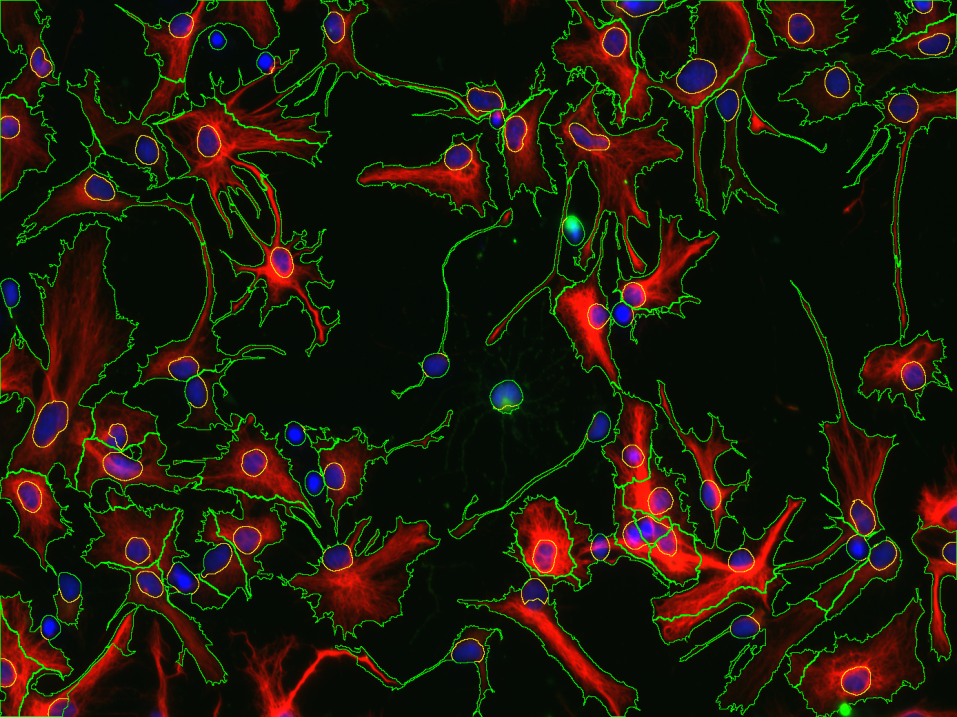
\includegraphics[width=0.4\textwidth]{figures/research/stem1.png}}
\subfigure[]{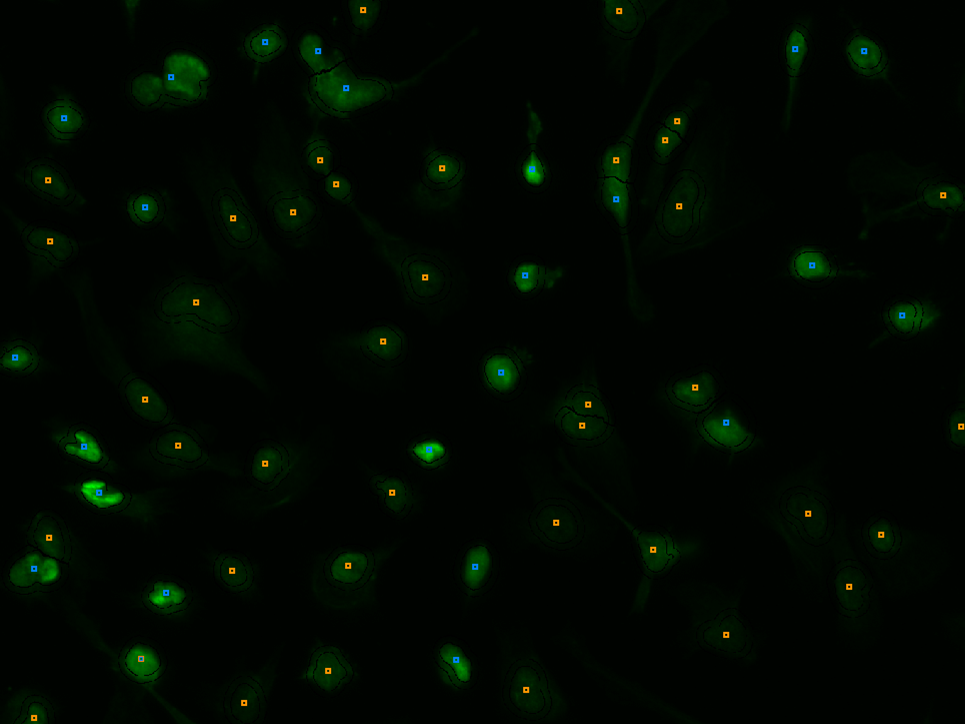
\includegraphics[width=0.4\textwidth]{figures/research/stem2.png}}
\caption{(a) Neural stem cells differentiating to astrocytes (red) and oligodendrocytes (green). Contours show segmented astrocytes and nuclei, using CellProfiler. Experiment by Tanja Paavilainen. (b) Cells from a glioma cell line expressing (blue marker) or not (orange marker) Oligodendrocyte transcription factor (OLIG2). Classifiaction obtained with CellProfiler Analyst. Experiment by Tobias Bergstr\"{o}m.}
\label{fig::stem_cells}
\end{figure*}

% GGG

\item
\label{proj:stemcells}
\textbf{SciLifeLab Cancer Stem Cell Program}\\
Carolina W\"{a}hlby, Ida-Maria Sintorn\\
\ppartners{Sven Nelander, Karin Forsberg-Nilsson, Irina Alafuzoff, Ulf Landegren, Anna Segerman, Tobias Sj\"{o}blom, Lene Urborn and Bengt Westermark, Department of Immunology, Genetics and Pathology and SciLifeLab, UU, Bo Lundgres, the Karolinska Institute and SciLifeLab, Stockholm, Rebecka J\"{o}rnsten, Chalmers, Gothenburg, and G\"{o}ran Hesselager, UU Hospital, Uppsala}
\ffunding{AstraZeneca-Science for Life Laboratory Joint Research Program}
\pperiod{1303--}
\aabstract{The SciLifeLab Cancer Stem Cell Program is a cross-platform initiative to characterize cancer stem cells (CSCs). Previously, the development of drugs targeting the CSC population in solid tumors has been curbed by the lack of valid cell model systems, and the complex genetic heterogeneity across tumors, factors that make it hard to assess new targets or predict drug responses in the individual patient. To solve these problems, our aim is to develop a biobank of highly characterized CSC cultures as a valid model of cancer heterogeneity. We will combine mathematical and experimental approaches, including image-based high-throughput cell screening, to define the spectrum of therapeutically relevant regulatory differences between patients. This will help elucidate mechanisms of action and enable accurate targeting of disease subgroups. During 2013, patient data was collected, and a number of primary cell lines were established. Cultured cells were exposed to a different treatments and doses (more than 2500 different treatments per cell line), and imaged by fluorescence as well as bright-field microscopy, and current focus is on extracting meaningful morphological descriptors from the image data.}

%HHH

\item \textbf{Endothelial Cell Segmentation of the Cornea of Human Eyes}\\
Bettina Selig, Cris Luengo\\
\ppartners{Bernd Rieger, Quantitative Imaging Group, Delft University
of Technology, Netherlands; Koen Vermeer, The Rotterdam Eye Hospital, The Netherlands}
\ffunding{S-faculty, SLU}
\pperiod{1103--}
\aabstract{The corneal endothelium plays a key role in maintaining the
transparency of the cornea. Because the cells in the endothelium do not
regenerate, the cell density decreases with age; this reduces its ability
to maintain the processes needed to keep the cornea transparent. Thus, being
able to measure this density in patients is very important. The endothelium
can be imaged by specular microscopy or by confocal scanners, and measurements
can be obtained manually, automatically with manual corrections, or fully
automatically with current software (e.g., Nidek's NAVIS). Unfortunately, the
results of the automatic methods are often useless, especially at low cell
densities. Together with the Rotterdam Eye Hospital, we have developed a fully
automatic method to segment individual cells in the corneal endothelium. The
result of the method (see Figure~\ref{fig:cornea}) can be used to determine
the cell density, but also other parameters of interest, like pleomorphism
(cell shape) and polymegathism (cell size variation). Our segmentation method produces a segmentation that matches a manual segmentation reasonably well, for a wide range of cell densities and image qualities. These results will be
published during 2014.}

\begin{figure}[!htbp]
\centering
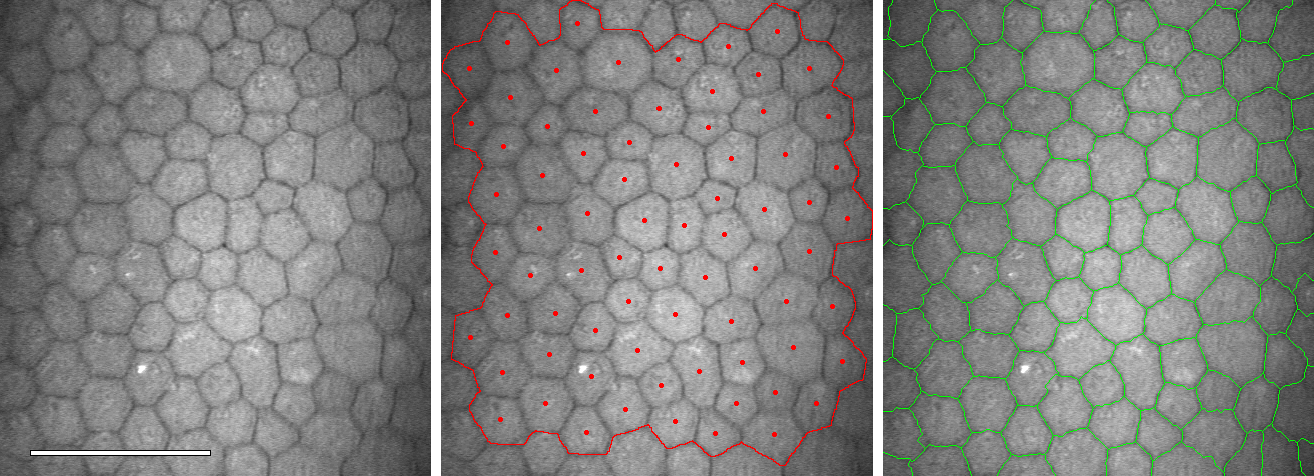
\includegraphics[width=.85\textwidth]{figures/research/corneal_epithelium.png}
\caption{\label{fig:cornea}
Slit-scanning confocal microscope image of the endothelium of a patient's cornea, with a manual marking used to determine cell density (red), and the result of our automated algorithm (green). The manual markings take about four minutes per image to do, whereas the algorithm finishes in less than half a minute and requires no interaction at all. The white bar indicates 100$\;\mu$m. The image is a typical example (i.e. the one with the nicest segmentation result).}
\end{figure}

%%% III

\item \textbf{CerviScan}\\
Ewert Bengtsson, Patrik Malm, Hyun-Ju Choi, Bo Nordin, Andrew Mehnert\\
\ppartners{Rajesh Kumar, Centre for Development of Advanced Computing (CDAC), Thiruvananthapuram, Kerala, India; K. Sujathan, Regional Cancer Centre, Thiruvananthapuram, Kerala, India}
\ffunding{Swedish Governmental Agency for Innovation Systems (VINNOVA); Swedish Research Council; SIDA}
\pperiod{0801--}
\aabstract{Cervical cancer is a disease that annually kills over a quarter of a million women world-wide. This number could be substantially reduced if women were regularly screened for signs of cancer precursors using the well established Pap-test. If detected early, these precursors can be treated with a very high rate of success. A problem with the Pap-test is that it requires highly trained cytotechnologists to perform thetime consuming visual analysis of the specimen. For over 50 years attempts to automate this process have been made but still no cost effective systems are available.

The CerviScan project is an initiative from the Indian government, managed by the research institute CDAC in cooperation with the Regional Cancer Centre (RCC) in Kerala and CBA in Sweden, aimed at creating a low cost, automated screening system. The system will reduce the number of cytotechnologists needed for population screening by identifying and removing specimen that are clearly normal. A prototype system has been created and used to screen over 1000 specimen (Fig. \ref{fig:cerviscan}). Initial classification results are promising but screening times are still about 10 times longer than what is realistic in a real screening setting. Plans for the next phase of the project, focusing on dedicated hardware, are under way and are currently awaiting the result of a funding application.
\clearpage
In Sweden, Ewert Bengtsson and Patrik Malm at CBA have in collaboration with Andrew Mehnert and students at MedTech West, Chalmers, been working on developing improved texture measures that are based on pseudo-3D information generated by imaging cells as focus stacks. This work is ongoing but has already led to two conference publications with a third manuscript on the way. Other work at CBA includes methods for nucleus segmentation, debris removal and field of view grading. Also, advanced procedural methods for synthetic Pap-smear image generation have been developed and published. Currently, a study aimed at determining the optimal optical resolution for a future system is taking place. Preliminary results of this study have been composed into a manuscript and submitted for conference publication.

The work has been summarized in a thesis dubbed "Image Analysis in Support of Computer-Assisted Cervical Cancer Screening" . The thesis was defended February 7, 2014 by Patrik Malm.}

\begin{figure}[!htbp]
\centering
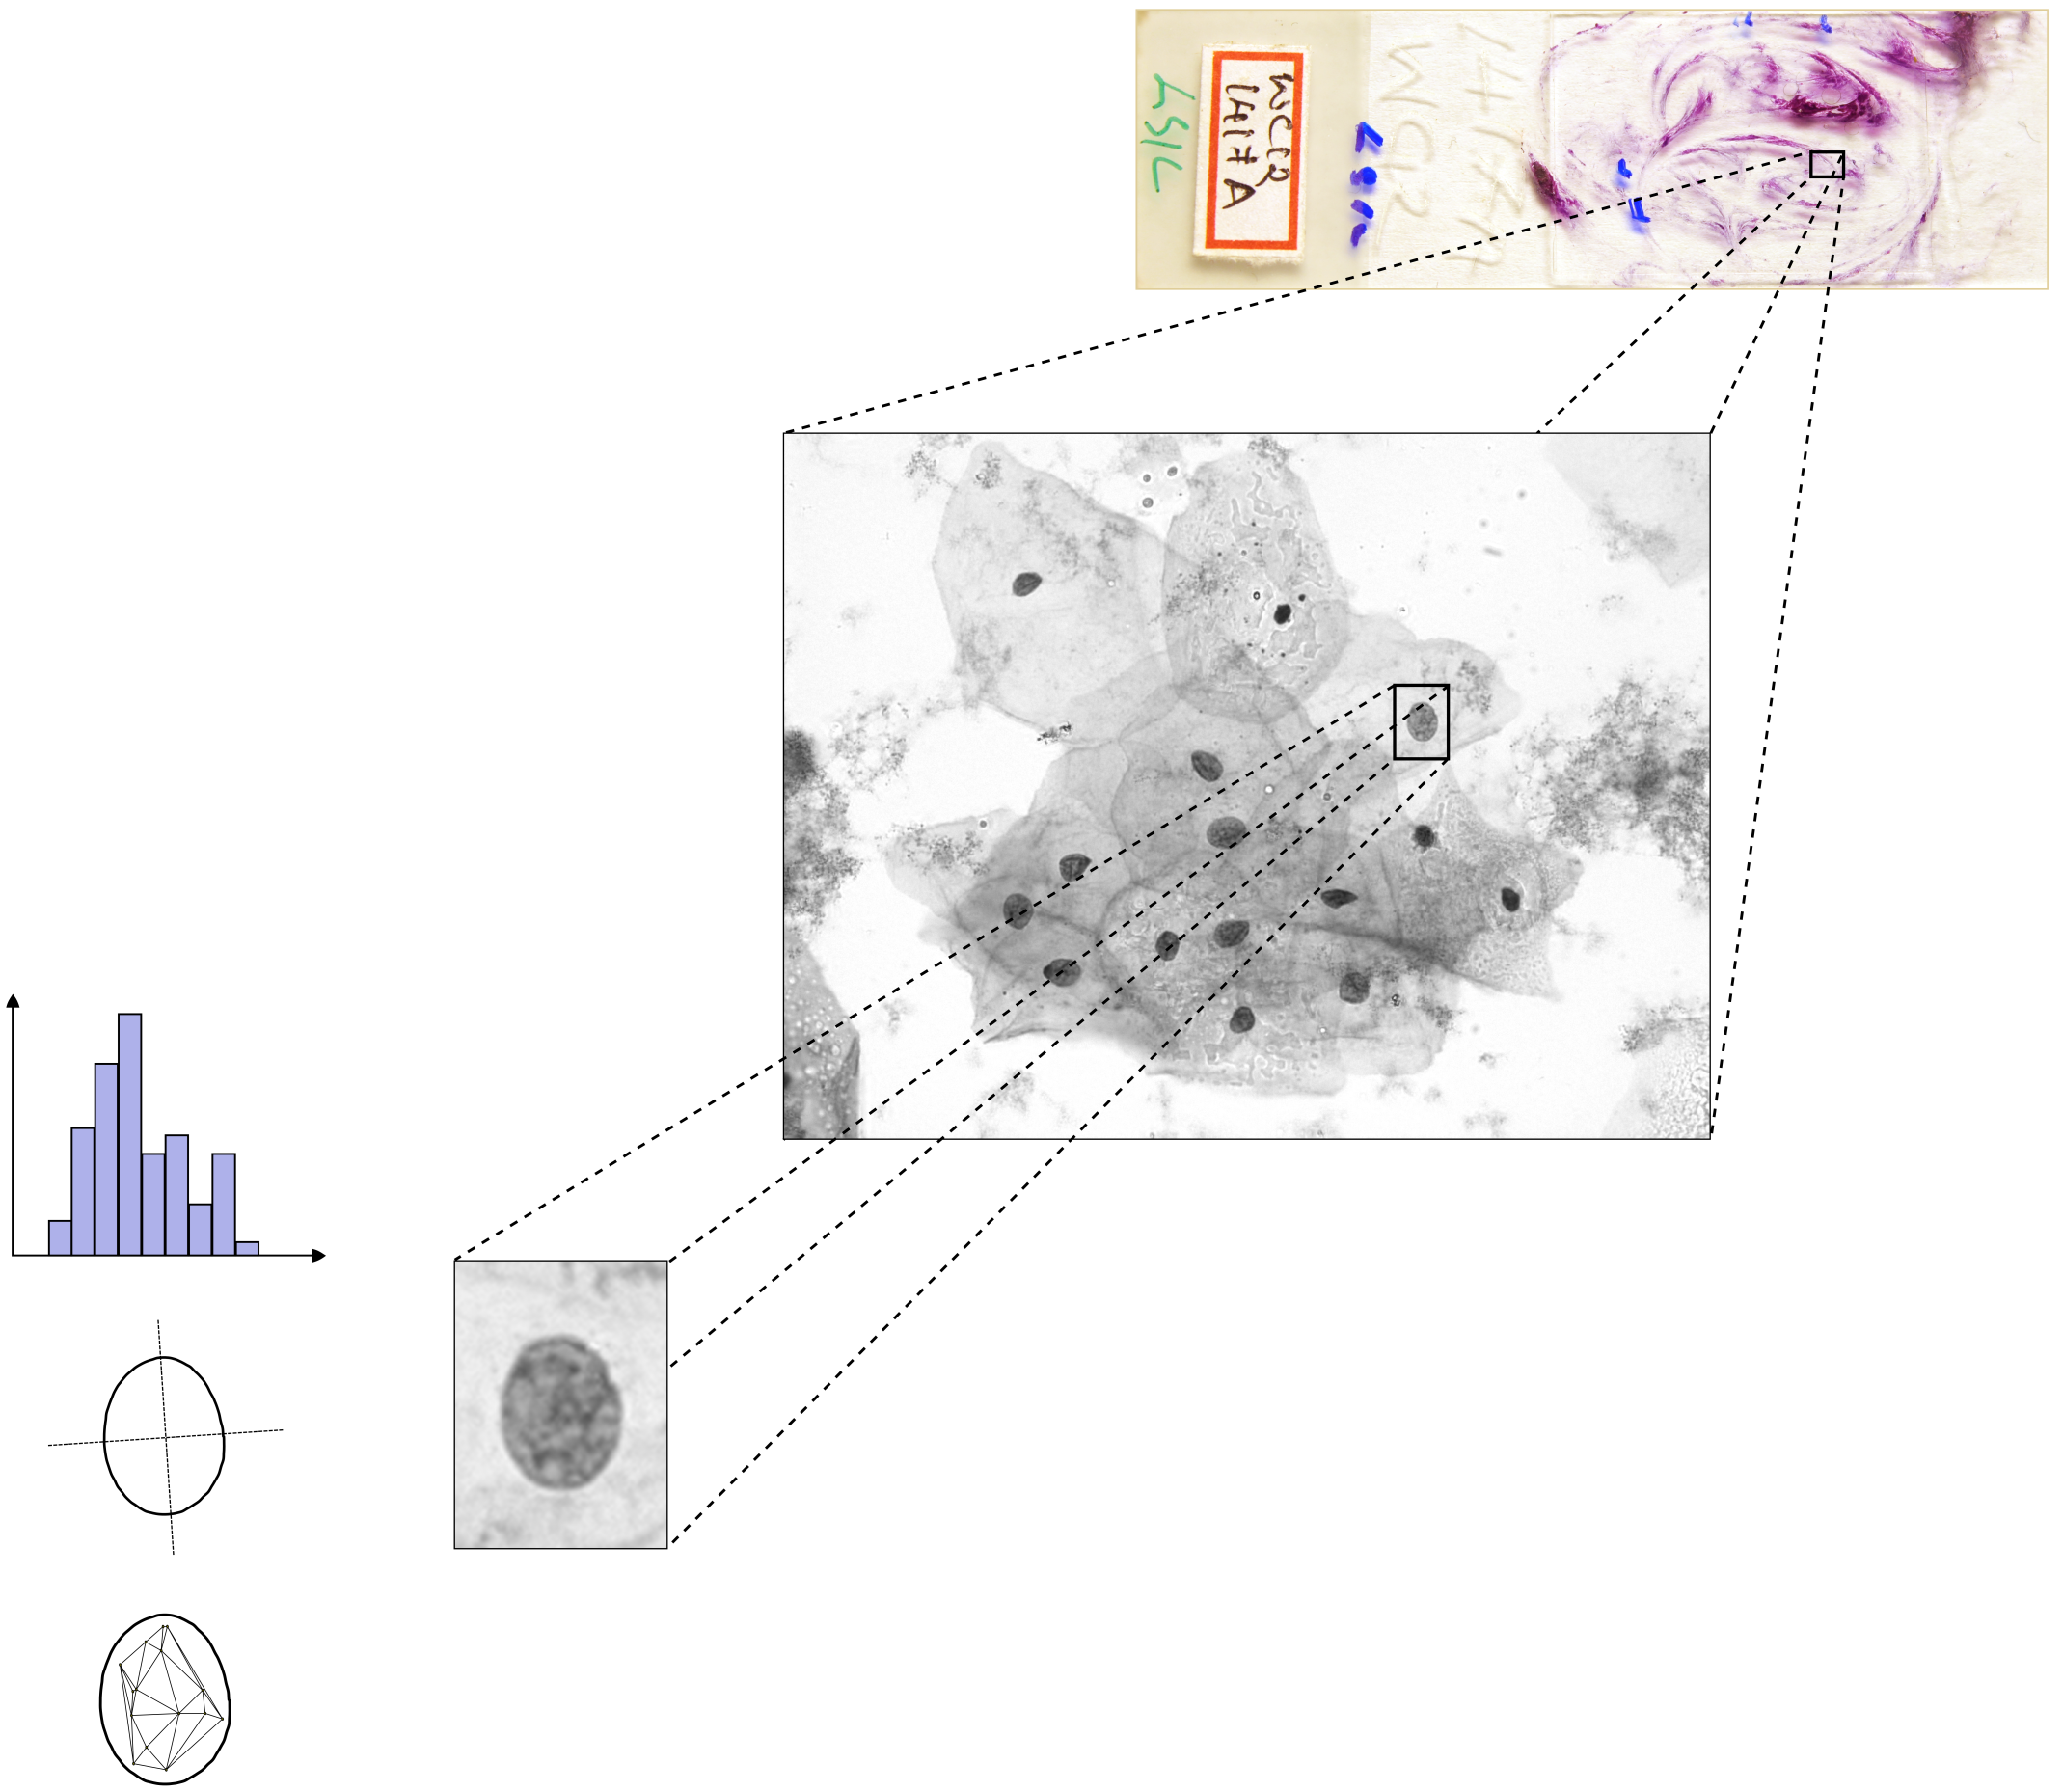
\includegraphics[width=0.70\textwidth]{figures/research/cerviscan.png}
\caption{\label{fig:cerviscan} The system developed in the CerviScan project will screen an entire specimen and within each field of view segment cervical cell nuclei that are visible. A series of structural and statistical measurements will then be acquired from these in order to determine if the specimen is normal or abnormal.}
\end{figure}

\newpage

%JJJ

\item \textbf{Automated Tissue Image Analysis using Pattern Recognition}\\
Ewert Bengtsson, Anders Hast, Jimmy Azar\\
\ffunding{TN-faculty, UU}
\pperiod{1001--}
\aabstract{The research was initially part of a VR supported project for grading
of prostate cancer; the final part of the research will focus on
analysis of samples from the Human Protein Atlas project aiming at
developing methods that can be used for computer assisted image
analysis of the huge database of images generated in that project.
In particular, image analysis methods will be developed for
histopathology, initially with applications to grading of prostate
cancer, but with extension to structural analysis of breast tissue
samples. The methods will be verified using paired antibody
evaluations.}

%KKK

\item \textbf{Detection and Classification of Malaria Infected Cells by LED Spectral Microscopy}\\
Carolina W\"{a}hlby\\
\ppartners{Jeremie Zoueu, Olivier Bagui, Dept.~Genie Electrique et Electronique, Institut National Polytechnique, Felix Houbhouet-Boigny, Cote d' Ivoire}
\pperiod{1109--}
\aabstract{This project aims to propose an effective optical device based on LED spectral microscopy, which will be low cost, fast and easy to use in the diagnosis of human malaria parasites, especially because the sample will not need any special preparation or staining and the data will be automatically processed to provide real-time diagnosis of the type of the parasite, the parasitic density and its age for an effective prescription. The collaborative project was initiated by a 3-month visit by Olivier Bagui, where we focused on the development of efficient segmentation methods for unstained images of blood cells. An efficient segmentation approach was developed using CellProfiler. Segmentation masks could thereafter be used to extract per-cell measurements for further exploration of spectral information on single cells.}

%%% LLL

\item 
\textbf{Studying Exocytosis by Time Lapse Microscopy}\\
Martin Simonsson, Carolina W\"{a}hlby\\
\ppartners{Anne Wuttke, Dept.~of Medical Cell Biology, UU}
\ffunding{SciLifeLab Uppsala, eSSENCE, VR junior research grant to CW }
\pperiod{1211-}
\aabstract{Insulin secreting cells perform exocytosis and this can be detected with a GFP-modified protein as an increase in fluorescence signal. Time-lapse sequences are acquired with a time interval of one second during one hour, observing changes in fluorescence signaling at different treatments of the cells. This results in huge data sets with more than 3000 images for a single experiment. The focus of this project is to extract relevant information from the image data and in an efficient way analyze and visualize the data. Preliminary results were presented in a PhD thesis by our collaborator Anne Wuttke, and a manuscript is in preparation.}

%MMM

\item 
\textbf{Tracking of Unstained Cells in Microfluidic Systems}\\
Sajith Kecheril Sadanandan, Martin Simonsson, Carolina W\"{a}hlby\\
\ppartners{Johen Kreuger, Sara Thorslund, Gradientech AB, Uppsala }
\ffunding{SciLifeLab Uppsala; eSSENCE; Dept.~of IT, UU}
\pperiod{1108--}
\aabstract{Tracking of cell movements in various cell culture setups is essential to many researchers in the life science sector. Gradientech AB, a Swedish biotech company, has developed CellDirector, a unique microfluidic system that academic researchers can use to study how concentration gradients of soluble proteins impact cell migration. The current project is focused on developing software for analyzing cell behavior and cell migration. The free open-source software CellProfiler developed at the Broad Institute will be used as a platform for a high-throughput system with automated high quality imaging, adapted for unlabeled cells, which are analyzed with regard to directionality of migration, speed, and acceleration. Apart from analyzing cell migration, the cell tracking aims at producing lineages, where cellular events such as cell division and cell death can be scored for single cells. A graphical user interface for visualizing and editing tracks imported from CellProfiler has been developed. This will be used for manual feed back in an iterative parameter optimization process, which aims to improve the automatic tracking. The progress of the project was presented in the poster session at eSSENCE Academy 2013 workshop at Lund.}

% NNN

\item 
\textbf{Segmentation and Tracking of E.coli Bacteria in Bright-Field Microscopy Images}\\
Sajith Kecheril Sadanandan, Carolina W\"{a}hlby\\
\ppartners{Johan Elf and David Fange, Dept.~of Cell \& Molecular Biology, UU}
\ffunding{SciLifeLab Uppsala, eSSENCE, VR junior researcher grant to CW}
\pperiod{1210--}
\aabstract{Time-lapse microscopy is used to study the cellular and molecular processes in live cell experiments. Tracking of live cells and analysis of their spatiotemporal behavior is a common task in many experiments. This project aims to segment E.coli bacteria and to track them over time to construct the cell lineage. Bacteria are grown in a microfluidic device developed at Elf lab, Uppsala, which enables the imaging of monolayer cells.  The unstained bright-field images of the cells are taken and a-priori information about the bacterial cells will be used to develop a system, which will have a GUI to set the parameters for proper segmentation and tracking. The results will be visually analyzed and the parameters are tuned. The optimized parameters will be used for the experiment to automatically analyze the data generated during the entire experiment.}

%OOO

\item % Analysis of microscopic biomedical images
\label{proj:cellsurfaceDiffusion}
\textbf{Modelling Diffusion on Cell Surfaces}\\
Ida-Maria Sintorn, Robin Strand \\
\ppartners{Ingela Parmryd, Dept.~of Medical Cell Biology, UU; Jeremy Adler, Dept.~Of Immunology, Genetics and Pathology, UU}
\ffunding{TN-faculty, UU; S-faculty, SLU; VINNMER programme, Swedish Governmental Agency for Innovation Systems}
\pperiod{1101--}
\aabstract{A cell surface is a highly irregular and rough. The surface
topography is however usually ignored in current models of the
plasma membrane, which are based on 2D observations of diffusion
that really occurs in 3D. In this project we model diffusion on
non-flat surfaces to explain biological processes occurring on the
cellsurface. During 2013, a poster was presented at Biophysical Society 2013 Annual Meeting, Philadelphia.}

%PPP

\item 
\textbf{Analysis of Male Reproductive Tract Morphology in Reproductive Toxicology}\\
Azadeh Fakhrzadeh, Cris Luengo, Gunilla Borgefors\\
\ppartners{Ellinor Sp\"{o}rndly-Nees,  Lena Holm, Dept.~of Anatomy, Physiology and Biochemistry, SLU}
\ffunding{SLU (KoN)}
\pperiod{1009--}
\aabstract{Reproductive toxicology is the study of chemicals and their effects on the reproductive system of humans and animals. In reproductive toxicology, there is a strong need to detect structural differences in organs that often have both a complex microscopic structure and function. This problem is further complicated because standard techniques are based on the examination of two-dimensional sections of a three-dimensional structure. The aim of this project is to develop methods to objectively describe microscopic structures of male reproductive organs and to test these in reproductive toxicology research. The project is comparative and  includes studies of organs from rooster and mink. We are developing automatic and interactive methods to analyze the relevant structures in the histology images of testis. We have constructed a semi-automatic method to delineate the epithelium cell layer in testicular tissue.
The cell nuclei are detected using the fast radial symmetry filter. A graph is constructed on top of the epithelial cells (Fig. \ref{testis}). Graph-cut optimization method is used to cut the links between cells of different tubules. Generating sperms in seminiferous tubules is a cyclic process, during which various generations of germ cells in epithelial layer undergo a series of developmental steps. This cycle can be subdivided into 12 different stages. We are currently developing a texture-based classification method to determine each tubule's stage.}

\begin{figure}[h]
\centering %\scalebox{1}{}
\includegraphics[width=0.8\textwidth]{figures/research/M1001cut.png}
 \caption{A graph constructed on top of Gata-4 marked germ cells.}
 \label{testis}
 \end{figure}

%QQQ

\item 
\textbf{Automated Classification of Immunostaining Patterns in Breast Tissue from the Human Protein Atlas}\\
Andreas K{\aa}rsn\"{a}s, Martin Simonsson, Carolina W\"{a}hlby, Robin Strand\\
\ppartners{Caroline Kampf, The Human Protein Atlas (HPA); Virginie Uhlmann,  Imaging Platform, Broad Institute of Harvard and MIT, Cambridge, Massachusetts MA, USA; S. Issac Niwas, P. Palanisamy, Dept.~of ECE, National Institute of Technology (NIT), Tiruchirappalli, India}
\ffunding{SciLifeLab Uppsala}
\pperiod{1201-1303}
\aabstract{The Human Protein Atlas (HPA) is an effort to map the location of all human proteins (\url{http://www.proteinatlas.org/}) and contains a large number of histological images of sections from human tissue. Methods for quantification of staining patterns in histopathology have many applications, ranging from antibody quality control to tumor grading. In this project we have tested a new method based on complex wavelets textural features as well as an approach inspired by WNDCHARM (Weighted Neighbor Distances using a Compound Hierarchy of Algorithms Representing Morphology) for classifying nuclear versus cytoplasmic staining. During 2013, a paper was published in Journal of Pathology Informatics.}

%RRR

\item % Analysis of microscopic biomedical images
\label{proj:CombatingCancer}
\textbf{Combating Breast Cancer by Digital Pathology}\\
Andreas K{\aa}rsn\"{a}s, Robin Strand, Carolina W\"{a}hlby, Ewert Bengtsson\\
\ppartners{Visiopharm, H{\o}rsholm, Denmark; Clinical Pathology Division, Vejle hospital, Vejle, Denmark}
\ffunding{NordForsk Private Public Partnership PhD Programme and Visiopharm}
\pperiod{0909--}
\aabstract{The results of analyses of tissue biopsies by pathologists are crucial for breast cancer patients. In particular, the precision of a patient's prognosis, and the ability to predict the consequences of various treatment opportunities before actually exposing the cancer patient, depend on the detection and quantification of biomarkers in tissue sections by microscopy. Experience from the last decade has revealed that manual detection and quantification of biomarkers by microscopy of tissue biopsies is highly dependent on the competencies and stamina of the individual pathologist. The aim of the present PhD project is to develop software-based algorithms that can facilitate the workflow and ensure objective and more precise results of the quantitative microscopy procedures in breast cancer.

During 2012, we worked on a project for verifying antibodies by comparing staining patterns in immune-stained histological images. The project was made in collaboration with the Human Protein Atlas project. We made a comparison of different methods for classifying staining patterns in histology. This work was presented at MICCAI'12 in Nice. We also presented the \textit{vectorial minimum barrier distance}, a new method for computing gray-weighted distance transforms while incorporating vectorial data, at ICPR'12 in Tsukuba, Japan. 

Early 2013, we started a new project aimed at developing a new method for registering histological images of consecutive sections with different staining. The project resulted in an article about multimodal registration using locally rigid transforms. The article is currently under review. In 2013, we also finished a journal article presenting a histopathological tool for sub-cellular quantification. The article was accepted early 2014 for publication in the journal \textit{Computer methods in Biomechanics and Biomedical Engineering: Imaging \& Visualization.}}

%SSS

\item 
\textbf{Automatic, Quantitative Malignancy Grading of Prostate Cancer using Image Analysis}\\
Ingrid Carlbom, Christophe Avenel\\
\ppartners{Christer Busch and Anna Tolf, Department of Immunology, Genetics and Pathology, University Hospital}
\ffunding{The Swedish Research Council, Hillevi Fries Research Fund}
\pperiod{1001--}
\aabstract{Gleason grading is the most widely used system for determining the severity of prostate cancer. The Gleason grade is determined visually under a microscope from prostate tissue that is most often stained with Hematoxylin-Eosin (H\&E).

\begin{figure}[!htbp]
\centering
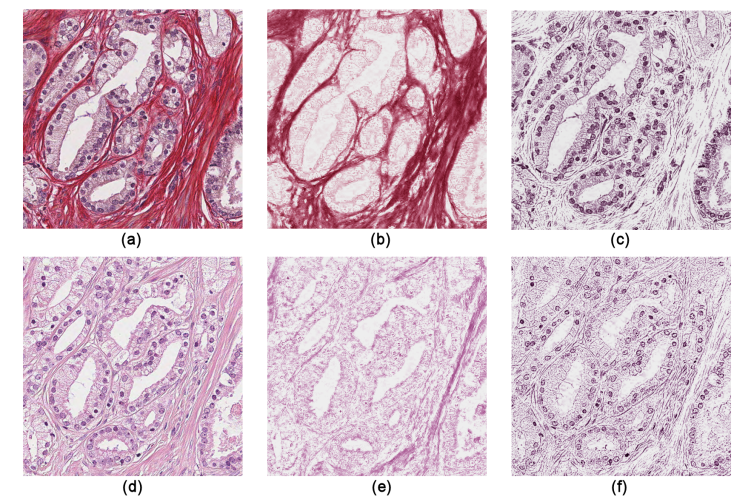
\includegraphics[width=.95\textwidth]{figures/research/prostate2.png}
\caption{Results of color decomposition: (a) original tissue image stained with Sir-Htx, (b) stroma density map, and (c) epithelial density map; (d) original tissue image stained with H\&E, (e) stroma density map, and (f) nuclei density map. \label{fig:prostate2}}
\end{figure}

\textit{Stain for blind color decomposition} In an earlier study we demonstrated that H\&E is not ideal for machine learning applications, but that other stains, such as Sirius-hematoxylin (Sir-Htx), may perform better. This year we demonstrated the advantages of this stain over H\&E for blind color decomposition (Fig. \ref{fig:prostate2}). When compared to ground truth defined by an experienced pathologist, the relative root-mean-square errors of the color decomposition mixing matrices for Sir-Htx are better than those for H\&E by a factor of two, and the Pearson correlation coefficients of the density maps resulting from the decomposition of Sir-Htx-stained tissue gives a 99\% correlation with the ground truth. Qualitative examples of the density maps confirm the quantitative findings and illustrate that the density maps will allow accurate segmentation of morphological features that determine the Gleason grade.
\newpage
\textit{Identification of epithelial nuclei} From the epithelial density map, resulting from the blind color decomposition of Sir-Htx-stained prostate tissue, we used a marked point process to segment the epithelial nuclei (Fig. \ref{fig:prostate3}). This enables us to extract nuclei as individual, joint, or overlapping objects generally without discarding overlapping parts and therefore without major loss in segmentation precision. The algorithm, which was originally developed for breast cancer tissue nuclei identification, uses simulated annealing combined with a "birth and death" process to find the best match with the density map, and was adapted to prostate tissue by pre-and-post processing methods.

\textit{Database of images from whole mount sections} We have created two online tools in order to build a database of graded images. The image selection tool is based on OpenSeaDragon (an open-source, web-based viewer for zoomable images) and facilitates the selection of small images from whole mount sections. With this tool we are building an image database where each image has a dominant pattern that represents for example one Gleason grade, benign tissue, stroma, or artifacts such as a tear in the tissue. The grading tool allows multiple pathologists to grade and comment on the previously selected images, without seeing each other grades, and is a basis for a consensus-graded database for developing and testing automatic Gleason grading algorithms (Fig. \ref{fig:prostate4}).} 

\begin{figure}
\centering
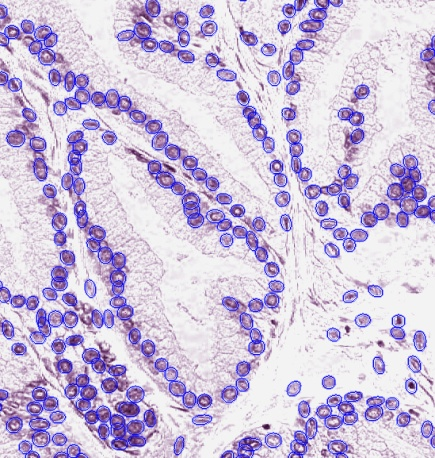
\includegraphics[width=.5\textwidth]{figures/research/prostate3.jpg}
\caption{Epithelial nuclei identified by the marked point process. \label{fig:prostate3}}
\end{figure}

\begin{figure}
\centering
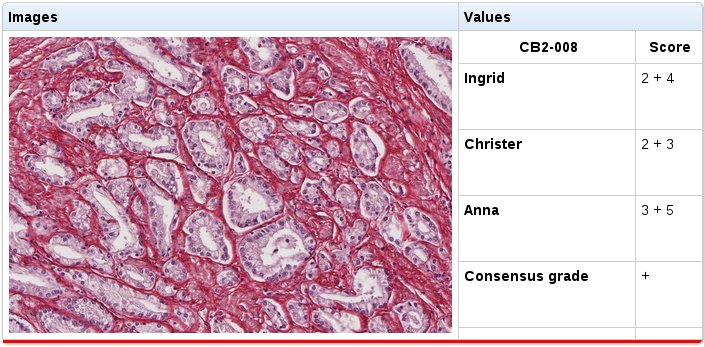
\includegraphics[width=.9\textwidth]{figures/research/prostate4.jpg}
\caption{Example of a sub-section of a whole-mount tissue section with three individual scores. \label{fig:prostate4}}
\end{figure}

%TTT
\newpage

\item 
\textbf{Automated Quantification of Zebrafish Tail Deformation for High-throughput Drug Screening}\\
Omer Ishaq, Alexandra Pacureanu, Carolina W\"{a}hlby\\
\ppartners{Joseph Negri, Mark-Anthony Bray, Randall T. Peterson, Broad Institute of Harvard and MIT}
\ffunding{SciLifeLab Uppsala}
\pperiod{1203--1304}
\aabstract{Zebrafish (\emph{Danio rerio}) is an important model organism in biomedical research due to its ease of handling and translucent body and consequently many human disease models have been established in the Zebrafish. Zebrafish embryos undergo spinal deformation upon exposure to chemical agents, such as Camptothecin (Cpt), that inhibit DNA repair. We are developing automated image-based quantification of spine deformation enabling whole-organism based assays for use in early-phase drug discovery campaigns. Our automated method for accurate high-throughput measurement of tail deformations in multi-fish micro-plate wells generates refined medial representations of partial tail-segments. Subsequently, these disjoint segments are analyzed and fused to generate complete Zebrafish tails (Fig. \ref{fig::zebrafish_curvature}). Based on these estimated tail curvatures we reach a classification accuracy of 91\% on individual animals as compared to known control treatment. This accuracy is increased to 95\% when combining scores for fish in the same well. A paper describing the methods and results was published and presented at the International Symposium for Biomedical Imaging (ISBI) in April 2013.}

\begin{figure*}[!htbp]
\centering
\subfigure[]{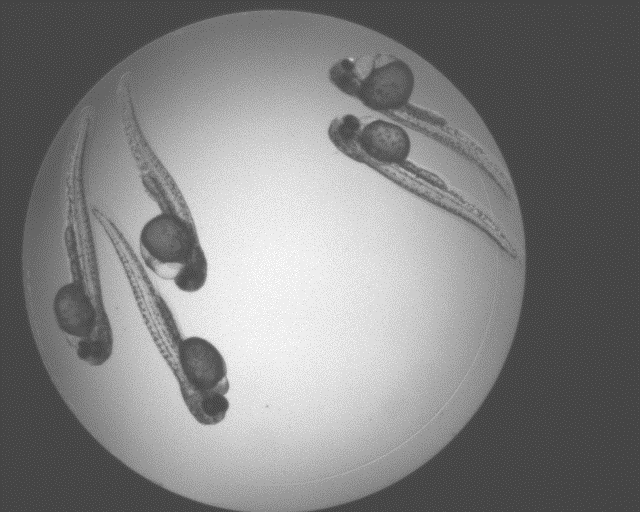
\includegraphics[width=0.3\textwidth]{figures/research/curvature1.png}}
\subfigure[]{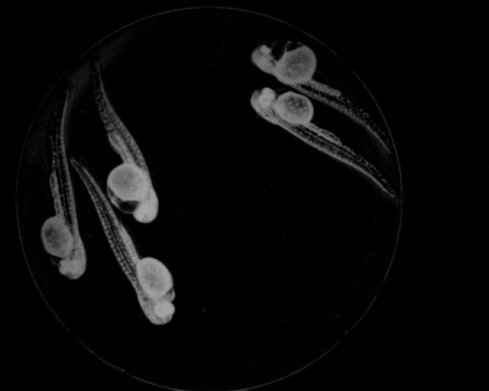
\includegraphics[width=0.3\textwidth]{figures/research/curvature2.png}}
\subfigure[]{
\includegraphics[width=0.3\textwidth]{figures/research/curvature3.png}}

\subfigure[]{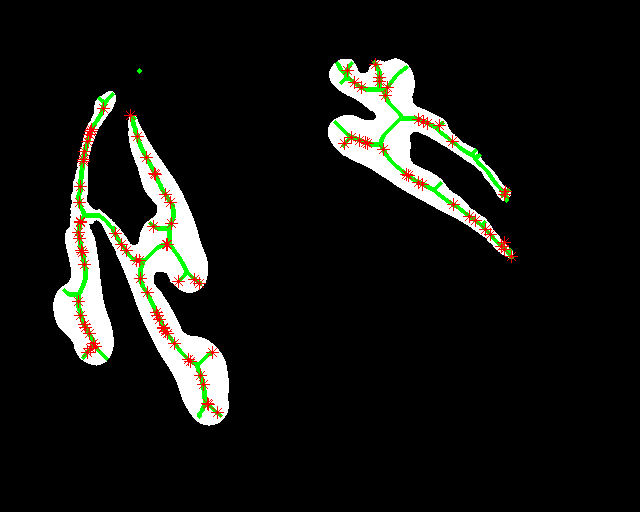
\includegraphics[width=0.3\textwidth]{figures/research/curvature4.png}}
\subfigure[]{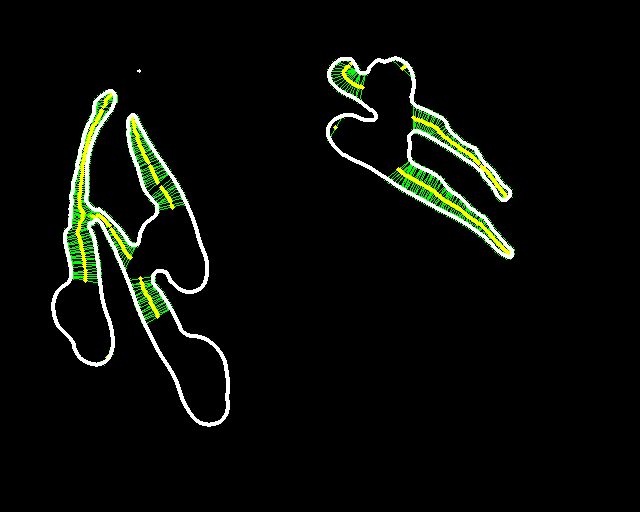
\includegraphics[width=0.3\textwidth]{figures/research/curvature5.png}}
\subfigure[]{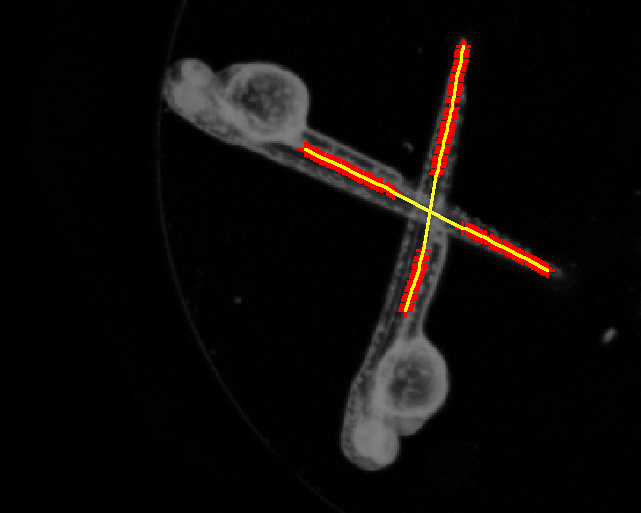
\includegraphics[width=0.3\textwidth]{figures/research/curvature6.png}}
\caption{Steps for curvature extraction: (a) An input image; (b) After illumination correction; (c) Binary image after smoothing and thresholding; (d) Computed medial axes (highlighted in green) and seed-points (highlighted in red); (e) Refined medial axes (highlighted in yellow); (f) Medial axis fusion: the red lines represent tail-segments fused together to yield the complete tails (shown in yellow).}
\label{fig::zebrafish_curvature}
\end{figure*}

%UUU

\item 
\textbf{Quantification of Zebrafish Lipid Droplets}\\
Petter Ranefall, Carolina W\"{a}hlby\\
\ppartners{Marcel den Hoed, Manoj Bandaru, Erik Ingelsson, Department of Medical Sciences and SciLifeLab, UU}
\ffunding{SciLifeLab Uppsala}
\pperiod{1308--}
\aabstract{The aim of this project is to identify novel targets for the therapeutic intervention of coronary artery disease. This is done by following-up results from genome-wide association studies in epidemiological studies using a zebrafish model system.  Using image analysis we try to identify and characterize causal genes within loci that have so far been identified as associated with coronary heart disease by (high-throughput) screening of atherogenic processes in wildtype and mutant zebrafish, both before and after feeding on a control diet or a diet high in cholesterol. Using confocal microscopy we can image fat accumulation in the zebrafish (Fig. \ref{fig:hamid}).}

\begin{figure}[!htbp]
\centering
\subfigure[]{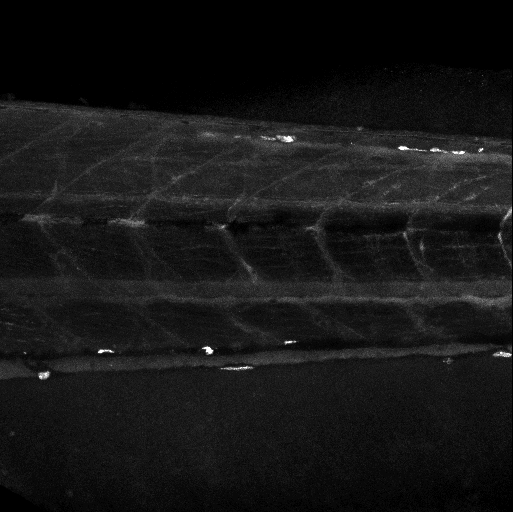
\includegraphics[width=44mm,height=44mm]{figures/research/lipid1.png}}
\subfigure[]{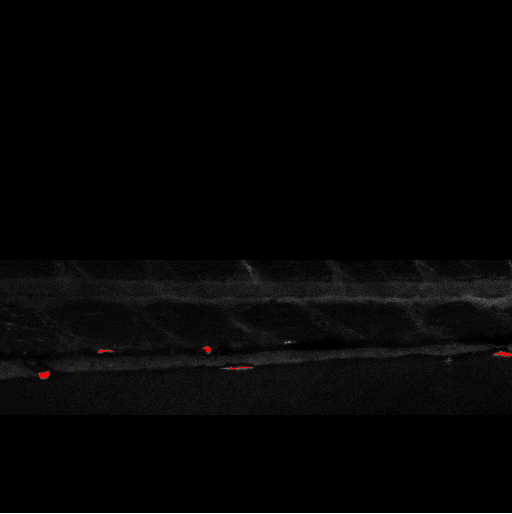
\includegraphics[width=44mm,height=44mm]{figures/research/lipid2.png}}
\caption{\label{fig:hamid}
The image to the left is a maximum projection of the zebrafish image volume, and the image to the right shows the detected stationary lipids in red.}
\end{figure}

%VVV

\item \textbf{Optical Projection Tomography}\\
Alexandra Pacureanu, Omer Ishaq, Carolina W\"{a}hlby\\
\ppartners{Amin Allalou, Izolde AB, Uppsala; Johan Ledin, Evolutionary Biology Centre, Zebrafish platform, SciLifeLab Uppsala; Jos Buijs, Ridgeview Uppsala, Carlos Pardo, Mehmet F. Yanik, Research Laboratory of Electronics, Massachusetts Institute of Technology, Cambridge, USA}
\ffunding{SciLifeLab Uppsala; TN-faculty, UU}
\pperiod{1009--}
\aabstract{Isotropic 3D imaging of biological specimens is instrumental for further breakthroughs in life sciences. Many biological specimens with high relevance for basic research, disease studies and drug discovery, such as model organisms or 3D cell cultures, are semi-transparent to visible light. This lead to the advent of the technique dubbed optical projection tomography (OPT). The 3D internal structure is revealed by the attenuation variations of the light traversing the specimen. In OPT transverse slices of the specimen are reconstructed from a set of angular projections and stacked together into a volumetric image. This method enables in vivo imaging of relatively large samples with high spatial resolution. A high-throughput platform for cellular resolution, in vivo OPT of zebrafish has been developed at MIT, Cambridge, USA. With this system we have shown that OPT of zebrafish embryos can provide 3D information enabling high-throughput screening of subtle phenotypic changes in relation to drug treatment, as published in Nature Communications in February 2013. However, OPT imaging systems in general are still quite sophisticated and costly. We are therefore developing a system for optical 3D isotropic imaging at microscopic scale, based on readily accessible hardware. The total price of the setup is kept under 1000 euros and the components can be easily obtained around the world. We have assembled the image acquisition system, acquired, and reconstructed images of zebrafish embryos (Fig. \ref{fig::tomography_fish}) and of 3D cell cultures (Fig. \ref{fig::tomography_cell}). We are complementing the simple hardware with open source computational tools, embedding algorithms for image alignment, correction and reconstruction. Our goal is to enable every life sciences research laboratory to have access to valuable 3D information on biological specimens.
In 2013, besides working on improving imaging of zebrafish embryos, we attempted to image 3D cell cultures with our system, in collaboration with Jos Buijs (Ridgeview). A human ovarian carcinoma cell line has been used to grow 3D cell cultures in borosilicate thin tubes. We also tested growing the cells in agar gels and performing a 'biopsy' to extract the cells and transfer them into borosilicate tubes for imaging. We presented a poster at IEEE International Symposium on Biomedical Imaging (ISBI), San Francisco, USA and a journal manuscript is under preparation.}

\begin{figure*}[!htbp]
\centering
\subfigure[]{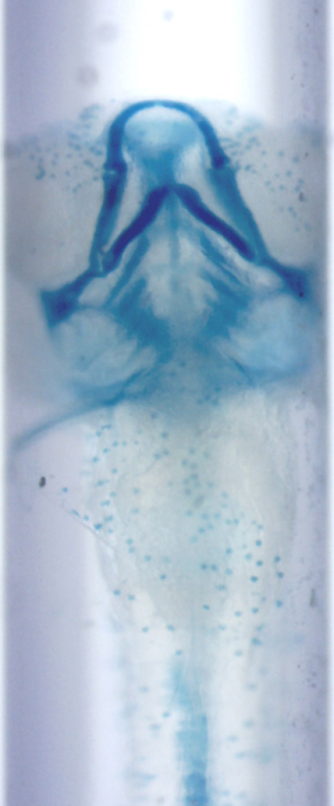
\includegraphics[width=26mm,height=55mm]{figures/research/zf1.png}}
\subfigure[]{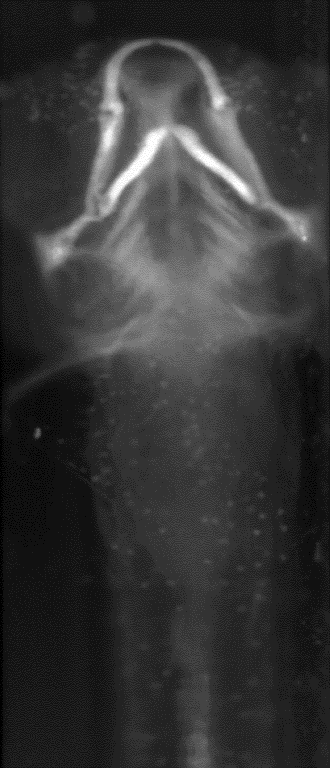
\includegraphics[width=26mm,height=55mm]{figures/research/zf2.png}}
\subfigure[]{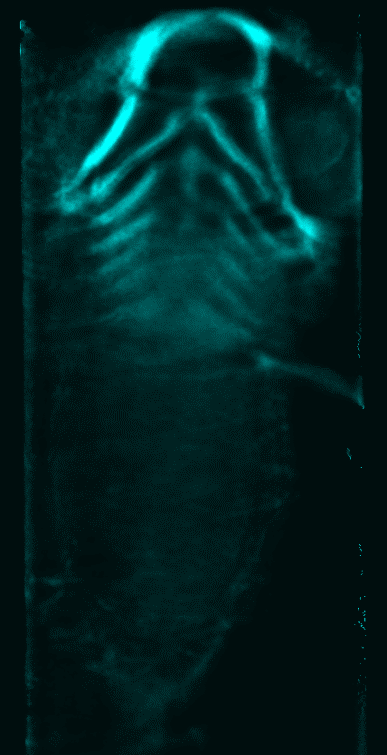
\includegraphics[width=26mm,height=55mm]{figures/research/zf3.png}}
\subfigure[]{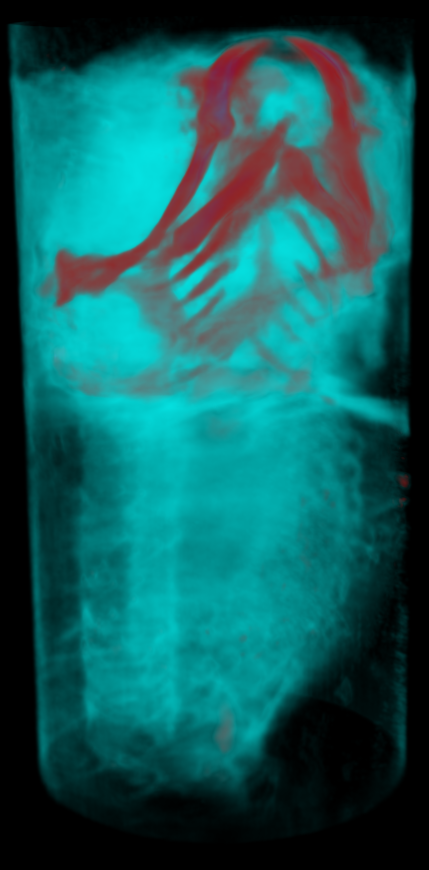
\includegraphics[width=26mm,height=55mm]{figures/research/zf4.png}}
\caption{(a) Recorded projection of a zebrafish embryo. (b) The projection after flat field correction. (c) Reconstructed frontal slice. (d) Volume rendering of the reconstructed image.}
\label{fig::tomography_fish}
\end{figure*}

\begin{figure*}[!htbp]
\centering
\subfigure[]{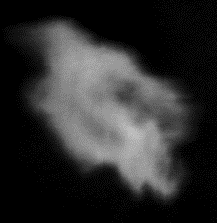
\includegraphics[width=40mm,height=40mm]{figures/research/cell1.png}}
\subfigure[]{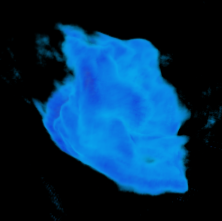
\includegraphics[width=40mm,height=40mm]{figures/research/cell2.png}}
\caption{(a) Projection of a 3D cell culture. (b) Volume rendering of the reconstructed image.}
\label{fig::tomography_cell}
\end{figure*}

%WWW
\item 
\textbf{Image-based Approaches for Drug Tablet Quality Assessment}\\
Ida-Maria Sintorn, Carolina W\"{a}hlby\\
\ppartners{Mark Nicholas, Mats Josefson, AstraZeneca, M\"{o}lndal, Sweden}
\ffunding{Pre-study grant from AIMDay Image, UU Innovation}
\pperiod{1204--1302}
\aabstract{It is known qualitatively that microstructural differences in solid dosage forms (e.g. tablets and inhalation powders) affect the performance of the medication. The microstructural differences are differences in the spatial distribution of active and inactive compounds. The aim of this project is to characterize these microstructural differences in order to determine whether imaging techniques such as CLSM (confocal laser scanning microscopy), wide-field fluorescence microscopy, and TOF-SIMS (Time-Of-Flight Secondary Ion Mass Spectroscopy) can reveal quantifiable differences in structure.  The problem was addressed using a combination of local intensity features and texture measurements (including granulometry, Zernike moments, and Haralick features), and measurements were correlated with tablet characteristics/treatments. Due to a relatively limited dataset, it was difficult to find statistically significant differences. The data was presented to AstraZeneca researchers in January 2013.}

% XXX
\newpage
\item
\label{proj:gigapixel}
\textbf{Tools for Analysis and Visualization of Giga-Pixel Sized  Slide-Scanner Images.}\\
Petter Ranefall, Alexandra Pacureanu, Carolina W\"{a}hlby\\
\ppartners{Mats Nilsson, Thomas Hauling, Marco Mignardi, Jessica Svedlund, Elin Lundin, Department of Biochemistry and Biophysics and SciLifeLab, Stockholm University.}
\ffunding{SciLifeLab}
\pperiod{1308--}
\aabstract{The aim is to create a tool for full resolution image analysis of large images, e.g. slide scanner data, with the possibility of visual examination and interaction at multiple resolutions. The tool is built on a free and open-source framework for visual examination at multiple resolutions with the option to toggle results on or off, such as segmentation masks, classification results, and tissue morphology measurements, using a map view with seamless zooming and panning capabilities, allowing for fast navigation between a full-tissue view and high-resolution sub-cellular observations (Fig. \ref{fig:gigapixel}). The aim is to also have an interface that enables visual/manual selection of regions of interest, target discovery, and understanding of novel spatial relationships within the tissue environment.}

\begin{figure}[!htbp]
\centering
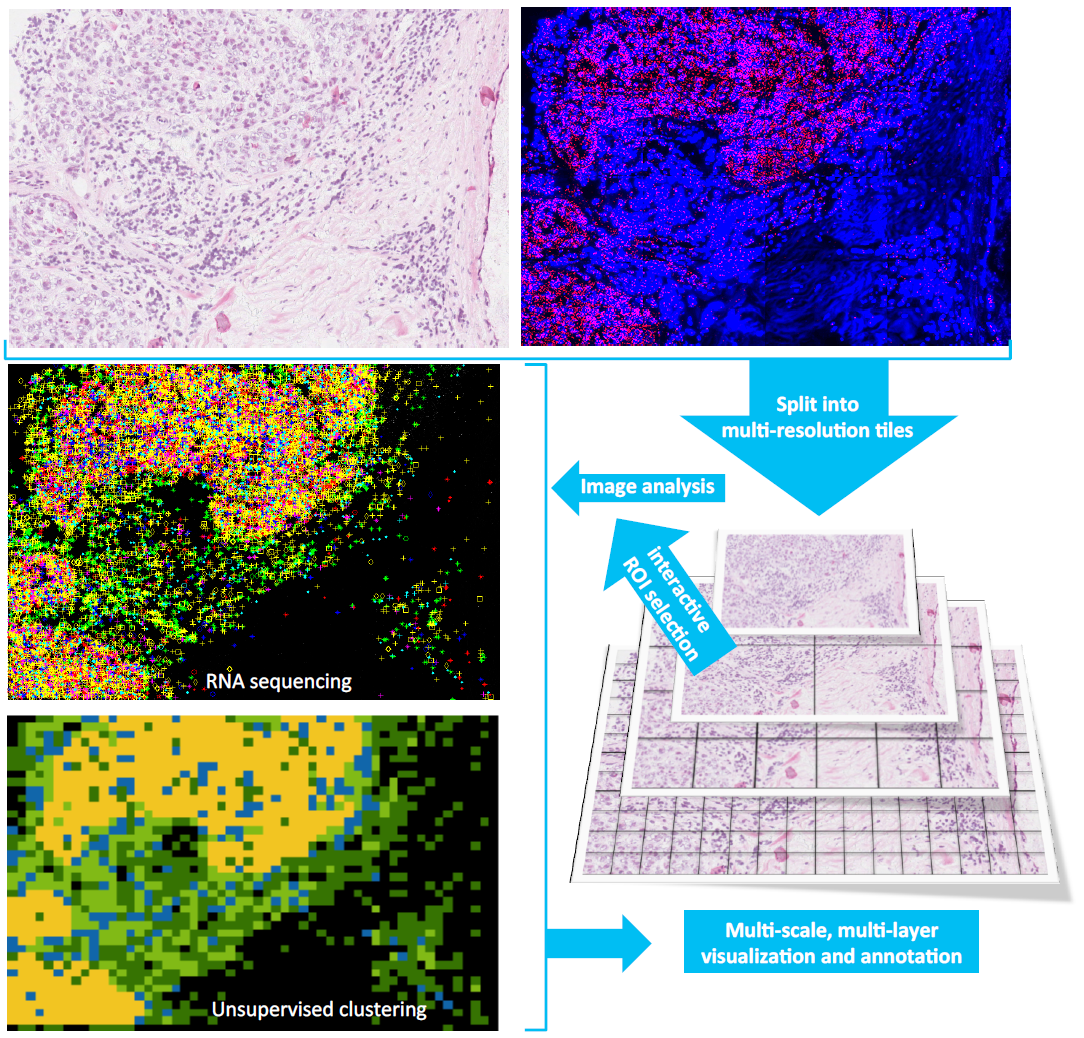
\includegraphics[width=0.8\textwidth]{figures/research/gigapixel.png}
\caption{\label{fig:gigapixel} A description of the workflow.} 
\end{figure}


\clearpage

%-------------------------------------------------------------------------------
%-------------------------------------------------------------------------------
%-------------------------------------------------------------------------------
%-------------------------------------------------------------------------------
%-------------------------------------------------------------------------------

\subsection{3D analysis and visualization}

%AAA

\item 
\label{proj:CMS}
\textbf{Haptics and its Applications to Medicine}\\
Ingrid Carlbom, Pontus Olsson, Fredrik Nysj\"{o}\\
\ppartner{Stefan Johansson (Division of Microsystems Technology, UU and Teknovest AB); Jan-Micha{\'e}l Hirsch, Dept.~of Surgical Sciences, Oral \& Maxillofacial Surgery, UU and Consultant at Dept.~of Plastic- and Maxillofacial Surgery, UU Hospital; Andreas Thor, Dept.~of Surgical Sciences, Oral \& Maxillofacial Surgery, UU Hospital; Andres Rodriguez Lorenzo, Department of Surgical Sciences, Plastic Surgery, UU Hospital; PiezoMotors AB.}
\ffunding{Dept.~of Surgical Sciences, Oral \& Maxillofacial Surgery, University Hospital; Thur\' eus Stiftelsen}
\pperiod{1401--}
\aabstract{This year we augmented the Uppsala Haptics-Assisted Surgery Planning (UHASP) system with virtual reconstruction of head and neck defects by fibula osteocutaneous free flaps (FOFF), including bone, vessels, and soft-tissue of the FOFF in the defect reconstruction. With the UHASP stereo graphics and haptic feedback, using patient-specific CT-angio data, the surgeons can plan bone resection, fibula design, recipient vessels selection, pedicle and perforator location selection, and skin-paddle configuration.

Two surgeons tested UHASP on four cases they had previously operated: three with composite mandibular defects and one with a composite cervical spine defect. (See Figure \ref{fig::haptics}) During the planning session, it became apparent that some problems encountered during the actual surgery could have been avoided. In one case, the fibula reconstruction was incomplete since the fibula had to be reversed and thus did not reach the temporal fossa. In another case, the fibula had to be rotated 180 degrees to correct the plate and screw placement in relation to the perforator. In the spinal case, difficulty in finding the optimal fibula shape and position required extra ischemia time. The surgeons found UHASP to be an efficient planning tool for FOFF reconstructions. The testing of alternative reconstructions to arrive at an optimal FOFF solution preoperatively potentially improves patient healing, function and aesthetics, and reduces operating room time.}

\begin{figure*}[!htbp]
\centering
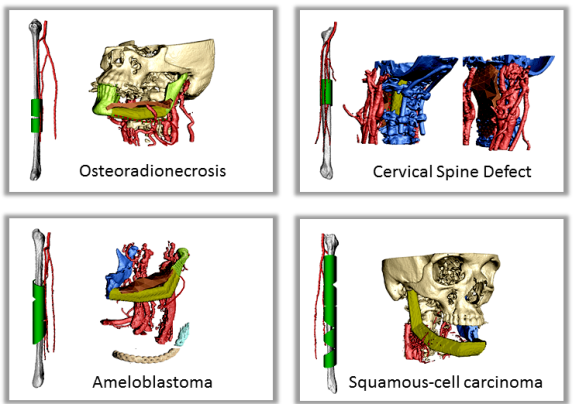
\includegraphics[width=0.9\textwidth]{figures/research/haptics.png}
\caption{The resulting plans for the four cases. The whole fibula with osteotomy positions and orientations are shown in relation to
surrounding vessels to the left of each case.}
\label{fig::haptics}
\end{figure*}

%----------------------------------------------------------------------------------------------------------------------------------------------

%BBB
\newpage
\item 
\textbf{ProViz -- Interactive Visualization of 3D Protein Images}\\
Lennart Svensson, Ida-Maria Sintorn, Ingela Nystr\"{o}m, Fredrik Nysj\"{o}, Johan Nysj\"{o}, Anders Brun, Gunilla Borgefors\\
\ppartners{Dept.~of Cell and Molecular Biology, Karolinska Institute; SenseGraphics AB}
\ffunding{The Visualization Program by Knowledge Foundation; Vaardal Foundation; Foundation for Strategic Research; VINNOVA; Invest in Sweden Agency; SLU, faculty funding}
\pperiod{0807--1412}
\aabstract{Electron tomography is the only microscopy technique that allows 3-D imaging of biological samples at nano-meter resolution. It thus enables studies of both the dynamics of proteins and individual macromolecular structures in tissue. However, the electron tomography images have a low signal-to-noise ratio, which makes image analysis methods an important tool in interpreting the images. The ProViz project aims at developing visualization and analysis methods in this area.

The project focus 2014 has been on finalizing and testing the methods and software as well as preparing the manuscript describing and demonstrating the ProViz software. Towards the end of the year, Lennart Svensson successfully defended his PhD thesis very closely linked to the ProViz project.}

% CCC
\newpage
\item 
\label{proj:MRI_optimal_lattices}
\textbf{Analysis and Processing of Three-Dimensional Magnetic Resonance Images on Optimal Lattices} \\
Elisabeth Linn\'{e}r, Robin Strand\\
%ppartner{Joel Kullberg, Dept.~of Radiology, Oncology and Radiation Science, UU}
\ffunding{TN-faculty, UU}
\pperiod{1005--}
\aabstract{Three-dimensional images are widely used in, for example, health care. With optimal sampling lattices, the amount of data can be reduced by 20-30\% without affecting the image quality, lowering the demands on the hardware used to store and process the images, and reducing processing time.

In this project, methods for image acquisition, analysis and visualization using optimal sampling lattices are studied and developed, with special focus on medical applications. The intention is that this project will lead to faster and better processing of images with less demands on data storage capacity. One of the goals of the project is to release open source software for producing, processing, analyzing and visualizing volume images sampled on BCC and FCC lattices, so as to make them readily available for potential users to explore on their own.
During 2014, the focus has been on distance transforms. Two reviewed conference papers exploring a graph-based implementation of the anti-aliased Euclidean distance transform have been published, and the work on the open source software is progressing.}

% DDD

\item 
\label{proj:MRI_registration}
\textbf{Registration of Medical Volume Images}\\
Robin Strand, Filip Malmberg\\
\ppartner{Joel Kullberg, H{\aa}kan Ahlstr\"{o}m, Dept.~of Radiology, Oncology and Radiation Science, UU}
\ffunding{Faculty of Medicine, UU}
\pperiod{1208--}
\aabstract{In this project, we mainly process magnetic resonance tomography (MR) images. MR images are very useful in clinical use and in medical research, e.g., for analyzing the composition of the human body. At the division of Radiology, UU, a huge amount of MR data, including whole body MR images is acquired for research on the connection between the composition of the human body and disease.

To compare volume images voxel by voxel, we develop image registration methods. For example, large scale analysis is enabled by image registration methods that utilizes, for example, segmented tissue (see, e.g., Project~\ref{project:medical_segmentation}) and anatomical landmarks. Based on this idea, we have developed Imiomics (imaging –omics) -- an image analysis concept, including image registration, that allows statistical and holistic analysis of whole-body image data (Figure \ref{fig:imiomics}). The Imiomics concept is holistic in three respects: (i) The whole body is analyzed, (ii) All collected image data is used in the analysis and (iii) It allows integration of all other collected non-imaging patient information in the analysis.}

\begin{figure*}[!htbp]
\centering
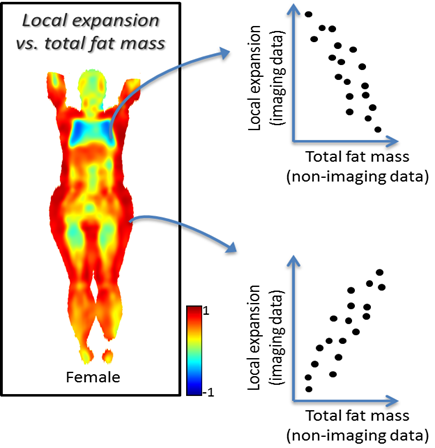
\includegraphics[width=0.9\textwidth]{figures/research/Imiomics_example.png}
\caption{\label{fig:imiomics} An illustration of a correlation map obtained by Imiomics. In this example, point-wise correlations between local tissue volume and body fat mass (measured by bioelectrical impedance analysis, BIA).} 
\end{figure*}

% EEE
\item 
\label{project:medical_segmentation}
\textbf{Interactive Segmentation and Analysis of Medical Images}\\
Filip Malmberg, Robin Strand, Ingela Nystr\"{o}m, Ewert Bengtsson\\
\ppartners{Joel Kullberg, H�kan Ahlstr�m, Department of Radiology, Oncology and Radiation Science, UU}
\ffunding{TN-faculty, UU}
\period 1106--\\
\aabstract{Three-dimensional imaging technique such as computed tomography (CT) and magnetic resonance imaging (MRI ) are now routinely used in medicine. This has lead to an ever increasing flow of high-resolution, high-dimensional, image data that needs to be qualitatively and quantitatively analyzed. Typically, this analysis requires accurate segmentation of the image. 

At CBA, we have been developing powerful new methods for interactive image segmentation. In this project, We seek to employ these methods for segmentation of medical images, in collaboration with the Department of Radiology, Oncology and Radiation Science (ROS) at the Uppsala University Hospital. 

During 2014, we published an article describing \emph{Smartpaint}, a tool for interactive segmentation of volume images. The SmartPaint software is publicly available and can be downloaded from \url{http://www.cb.uu.se/~filip/SmartPaint/}. To date, this software has been downloaded more than 500 times.} 

%\begin{figure}[!tb]
%\centering
%\includegraphics[width=1\textwidth]{figures/research/SP_screenshot.png}
%\caption{\label{fig:haptic} Screenshot from the \emph{Smartpaint} software for interactive segmentation of volume images, developed at CBA. A radiologist segments the liver in a CT image by interactively ``painting'' the segmentation using a brush tool.} 
%\end{figure}

% FFF

\item
\label{project:orbit_segmentation}
\textbf{Orbit Segmentation for Cranio-Maxillofacial Surgery Planning}\\
Johan Nysj\"{o}, Ida-Maria Sintorn, Ingela Nystr{\"o}m, Filip Malmberg\\
\ppartners{Jan Michael Hirsch, Andreas Thor, Johanna Nilsson, Dept.~of Surgical Sciences, UU Hospital; Roman Khonsari, Pitie Salpetriere Hospital, Paris, France; Jonathan Britto, Great Ormond Street Hospital, London, United Kingdom}
\ffunding{TN-faculty, UU}
\pperiod{0912--}
\aabstract{An important component in cranio-maxillofacial (CMF) surgery planning is to be able to accurately measure the extent of certain anatomical structures. The shape and volume of the orbits (eye sockets) are of particular interest. These properties can be measured in CT images of the skull, but this requires accurate segmentation of the orbits. Today, segmentation is usually performed by manual tracing of the orbit in a large number of slices of the CT image. This task is very time-consuming, and sensitive to operator errors. Semi-automatic segmentation methods could reduce the required operator time substantially. In this project, we are developing a prototype of a semi-automatic system for segmenting the orbit in CT images. The segmentation system is based on WISH, a software package for interactive visualization and segmentation that has been developed at CBA since 2003. WISH has been released under an open-source license and is available for download at \url{http://www.cb.uu.se/research/haptics}.

Our main focus during 2014 has been to continue our collaboration with surgeons from the Craniofacial Centre at Great Ormond Street Hospital, London, United Kingdom, in a project that aims to analyse the size and shape of the orbits in a large set of pre- and post-operative CT images of patients with congenital disorders. Our semi-automatic segmentation system has been used to rapidly segment the orbits in these datasets, and we have extended the system with automatic registration-based techniques for performing size and shape analysis of the segmented orbits. Abstracts about the ongoing work have been presented at medical conferences. We completed the size and shape analysis experiments for the study during the autumn and have now started to summarize the results in manuscripts.}

% GGG

\item 
\label{project:wrist_angle_measurements}
\textbf{Precise 3D Angle Measurements in CT Wrist Images}\\
Johan Nysj{\"o}, Filip Malmberg, Ingela Nystr{\"o}m, Ida-Maria Sintorn\\
\ppartners{Albert Christersson, Sune Larsson, Dept.~of Orthopedics, UU Hospital}
\ffunding{TN-faculty, UU}
\pperiod{1111--}
\aabstract{To be able to decide the correct treatment of a fracture, orthopedic surgeons need to assess the details about the fracture. One of the most important factors is the fracture displacement, particularly the angulation of the fracture. The wrist is the most common location for fractures in the human being. When a fracture is located close to a joint, for example, in the wrist,  the angulation of the joint line in relation to the long axis of the long bone needs to be measured. Since the surface of the joint line in the wrist is highly irregular, and since it is difficult to take X-rays of the wrist in exactly the same projections from time to time, conventional X-ray is not an optimal method for this purpose. In most clinical cases, conventional 2D angle measurements in X-ray images are satisfactory for making correct decisions about treatment, but when comparing two different methods of treatment, for instance, two different operation techniques, the accuracy and precision of the angle measurements need to be higher.

In this project, we are developing a system for performing precise 3D angle measurements in computed tomography (CT) images of the wrist. Our proposed system is semi-automatic; the user is required to guide the system by indicating the approximate position and orientation of various parts of the radius bone. This information is subsequently used as input to an automatic algorithm that makes precise angle measurements. We have developed a RANSAC-based method for estimating the long axis of the radius bone and a registration-based method (Figure \ref{fig:wrist}) for measuring the orientation of the joint surface of the radius. Preliminary evaluations have shown that these two methods together enable relative measurements of the dorsal angle in the wrist with sub-millimeter precision. During 2014, we performed a more extensive case study (involving 40 CT scan sequences of fractures wrists) to further evaluate the performance of our 3D angle measurement method and compare it with the conventional 2D X-ray measurement method. A manuscript about this study is under preparation.}

\begin{figure}[!htbp]
\centering
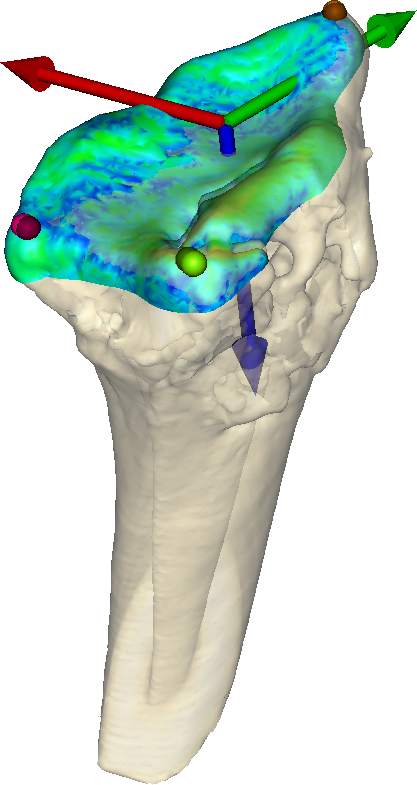
\includegraphics[height=0.9\textwidth, angle=90]{figures/research/wrist_2014.png}
\caption{\label{fig:wrist} Registration-based method for estimating the joint surface orientation in a fractured radius bone in the wrist. A template model of the joint surface is fitted to the target radius bone through landmark-guided surface registration, so that a local reference coordinate system of the template can be used to represent the joint surface orientation. The distance between the template and the joint surface is color-coded during the semi-automatic registration process.}
\end{figure}

% HHH

%\item \textbf{Ubiquitous Visualization in the Built Environment}\\
%Stefan Seipel, Fei Liu\\
%\ffunding{University of G\"{a}vle; TN-faculty, UU}
%\pperiod{110801--}%20150801}
%\aabstract{This research project in ubiquitous visualization deals with mobile visualization of spatial data in indoor and outdoor environments. Several key problems for robust mobile visualization are addressed such as spatial tracking and calibration, image based 2D and 3D registration and efficient graphical representations in mobile user interfaces. During 2013 we have devised a fasade region detection method by analyzing image profiles for repetitive patterns in street view images. These profiles are generated by scanning the hue channel of images along lines constructed with edge line segments and vanishing points. The work has been compiled into a paper titled "Detection of Fasade Regions in Street View Images from Split-and-Merge of Perspective Patches" and submitted to the International Conference on Computing and Computer Vision 2014. Meanwhile, we have also been exploring various image features to describe the detected fasade regions in order to identify which building is presented in a specific image.}

\newpage
\item
\label{proj:feione}
\textbf{Ubiquitous Visualization in the Built Environment}\\
Stefan Seipel, Fei Liu\\
\ppartner{Department of Industrial Development, IT and Land Management, University of G\"{a}vle}
\ffunding{University of G\"{a}vle; TN-faculty, UU}
\pperiod{1108--}
\aabstract{ This project deals with mobile visualization and augmented reality (AR) in indoor and outdoor environments. Several key problems for robust mobile visualization are addressed such as spatial tracking and calibration; image based 2D and 3D registration and efficient graphical representations in mobile user interfaces.

During 2014 two major lines of work have been carried out: Registration of thermal infrared and visible fa�ade images for augmented reality-based building inspection. Here, the problem of multi-modal image registration is addressed through identification of high-level (quadrilateral) features which model the shapes of commonly present fa�ade elements, such as windows (Fig. \ref{fig:regone}). These features are generated by grouping edge line segments with the help of image perspective information, namely, vanishing points. Our method adopts a forward selection algorithm for selecting feature correspondences needed to estimate the transformation model (Fig. \ref{fig:regtwo}). During the formation of the feature correspondence set, the correctness of selected feature correspondences at each step is verified through the quality of the resulting registration, which is based on the ratio of areas between the transformed features and the reference features. Part of this work has been published in the Journal of Image and Graphics. Other results of this work are currently prepared for publication.}

\begin{figure}[!htbp]
\centering
\includegraphics[width=0.8\textwidth]{figures/research/features.pdf}
\caption{\label{fig:regone} Selected control points for registration. Within an image, control points with the same color means they are from the same quadrilateral feature while across the images, the same color indicates correspondence.} 
\end{figure}

\begin{figure}[!htbp]
\centering
\includegraphics[width=0.8\textwidth]{figures/research/regiresult.pdf}
\caption{\label{fig:regtwo} Registration result showing the fusion of thermal infrared and visible images by alpha blending.} 
\end{figure}

Another activity in the project has been the development of a video-see through augmented reality system along with an experimental study on positioning accuracy in indoor augmented reality. In this work, a marker-based augmented reality application has been developed which displays construction elements (pipes) hidden inside walls as virtual models that are visually overlaid in real time upon video images of the real wall (Fig. \ref{fig:arcomp}). Using this application, we conducted a user experiment to find out how precise the localization of hidden structures in walls could be performed by the use of a video-see through augmented reality guidance system. Another objective was to investigate different factors that are influential on positioning accuracy, such as e.g. visual parallax and method for targeting (Fig. \ref{fig:arlab}). Experiment results have been gathered and as of now they are analyzed and prepared for publication. 

\begin{figure}[!htbp]
\centering
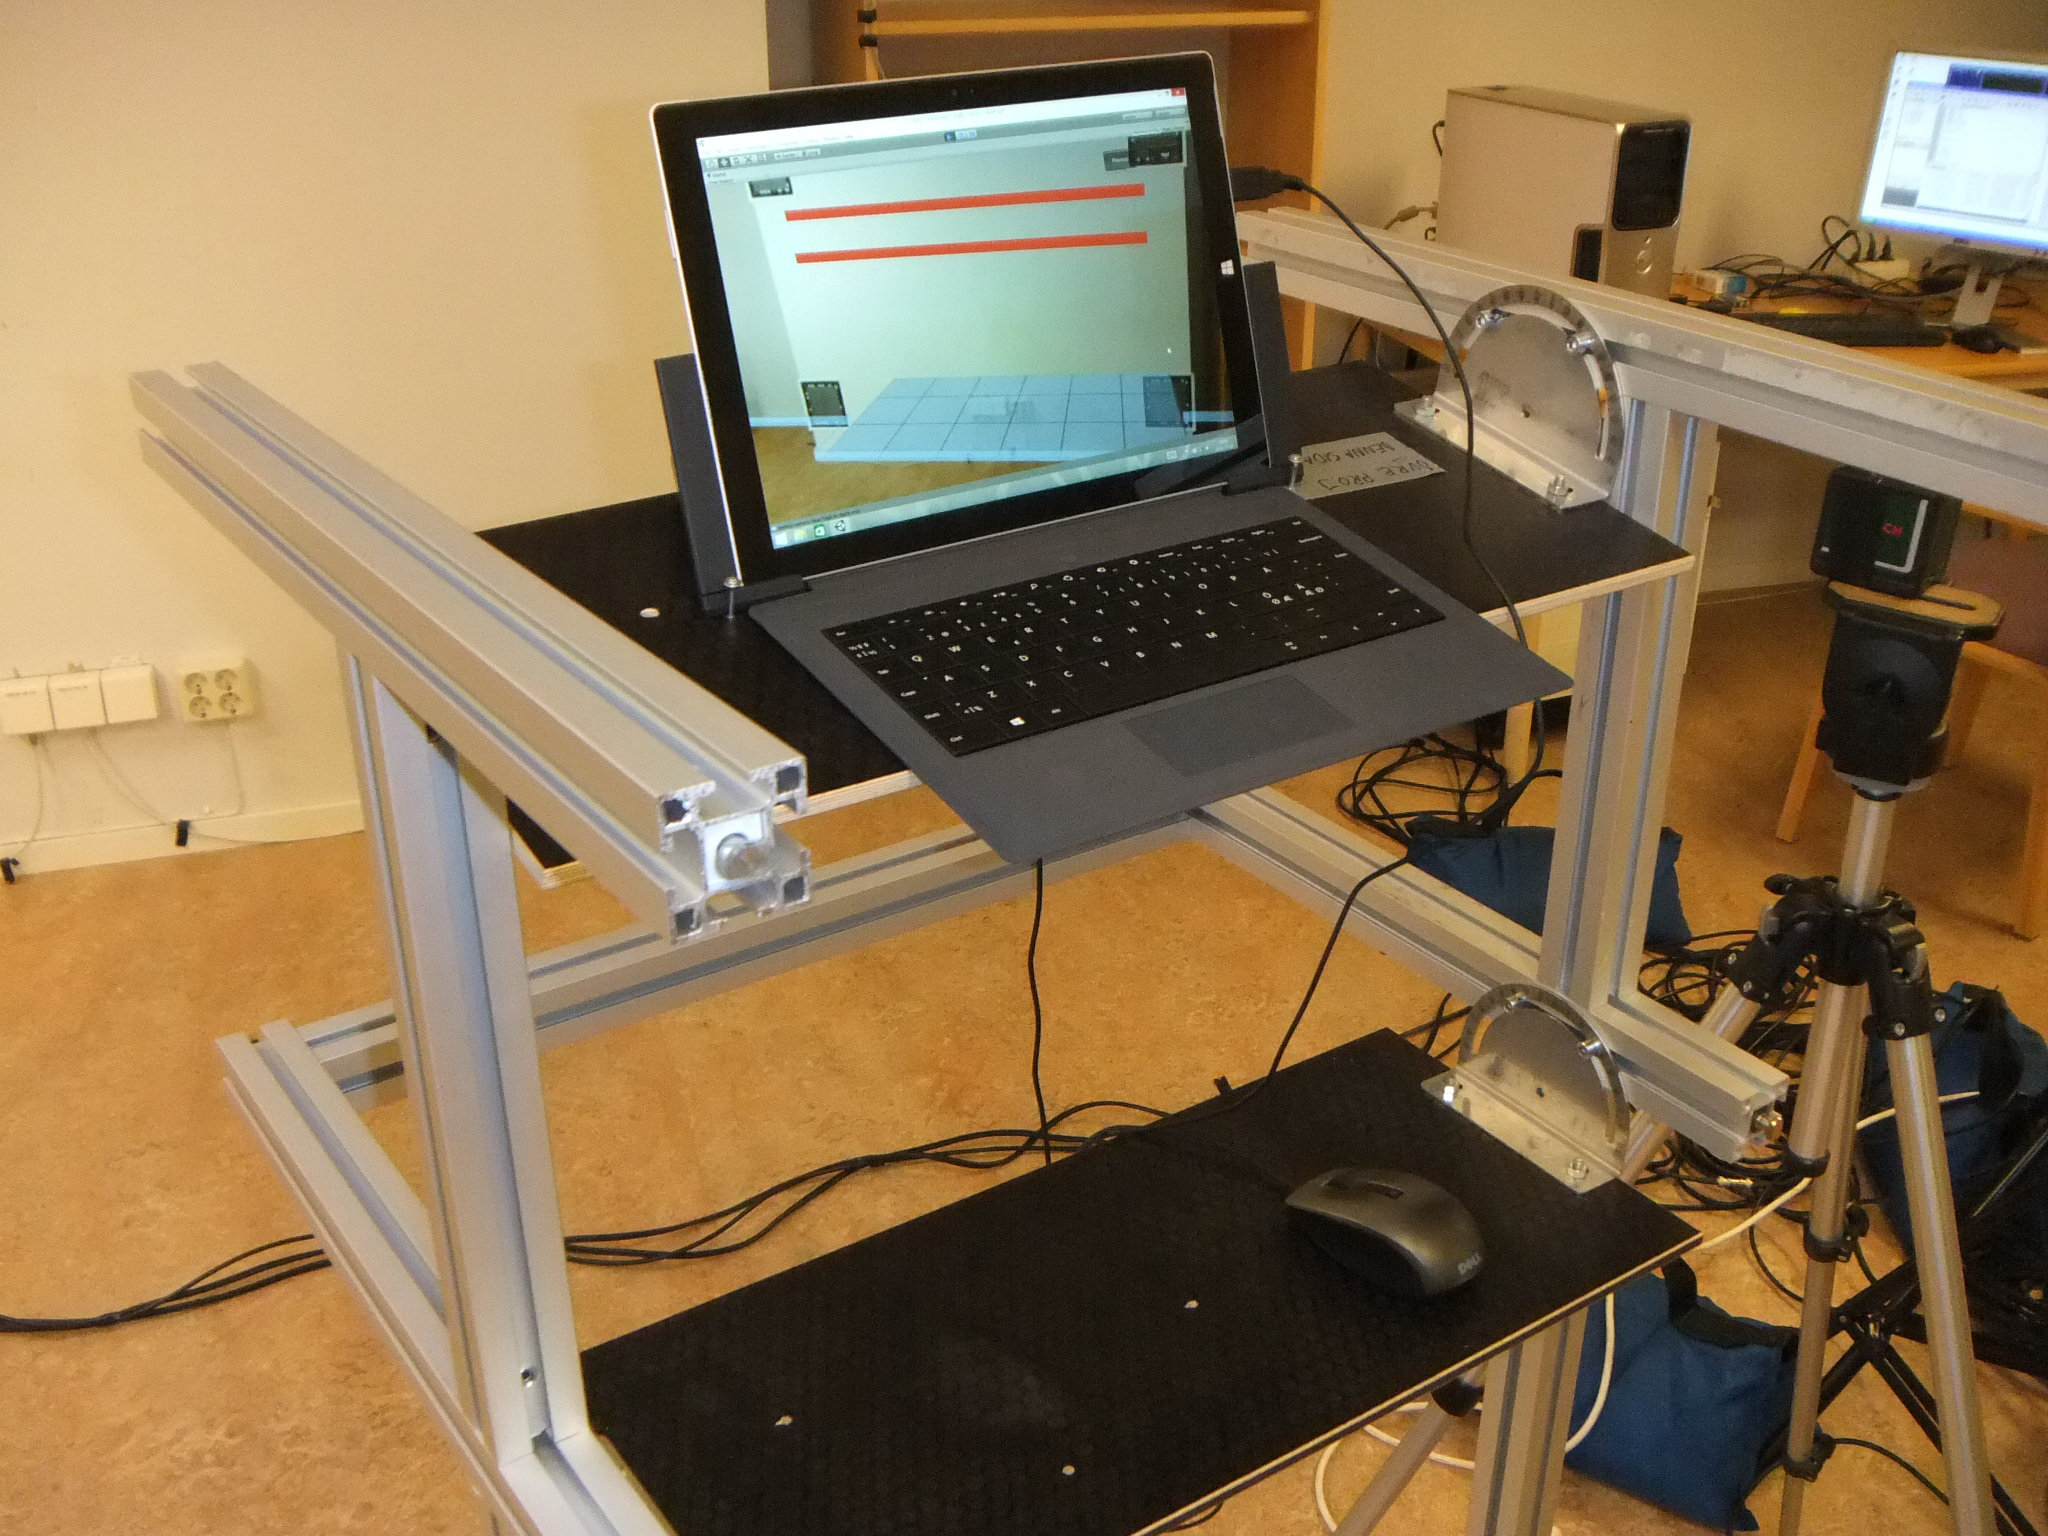
\includegraphics[width=0.8\textwidth]{figures/research/arapp.jpg}
\caption{\label{fig:arcomp} The augmented reality application running on the tablet.} 
\end{figure}

\begin{figure}[!htbp]
\centering
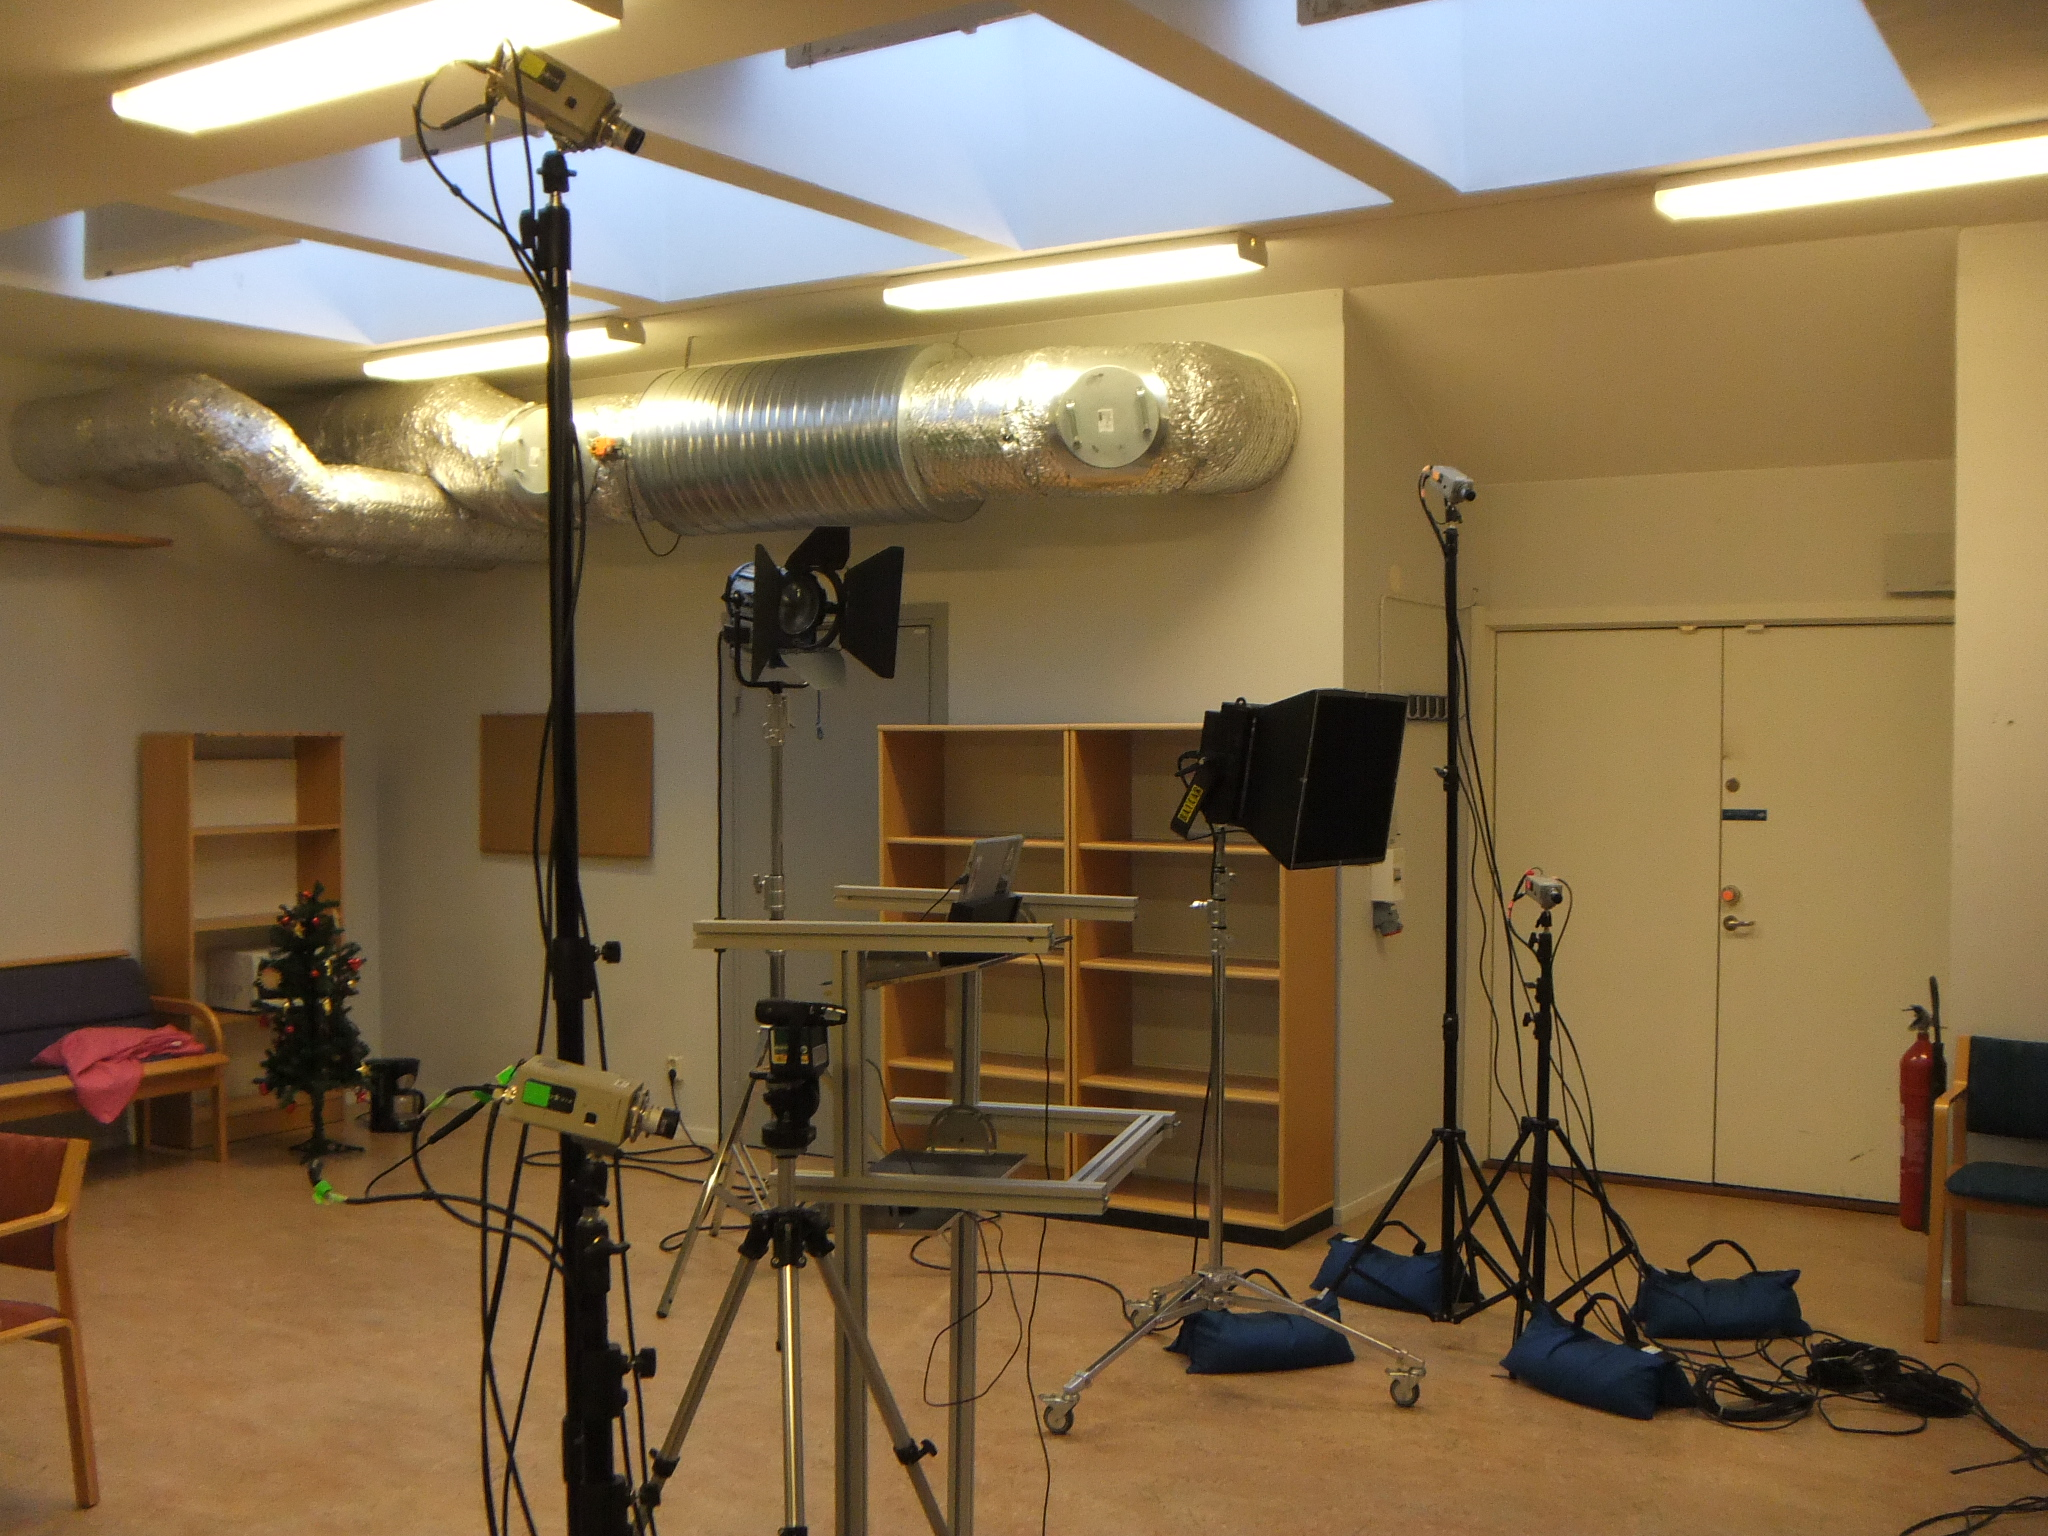
\includegraphics[width=0.8\textwidth]{figures/research/lab.jpg}
\caption{\label{fig:arlab} Eexperimental setup.} 
\end{figure}

\clearpage

%-------------------------------------------------------------------------------
%-------------------------------------------------------------------------------
%-------------------------------------------------------------------------------
%-------------------------------------------------------------------------------
%-------------------------------------------------------------------------------

\subsection{Theory: discrete geometry, mathematical morphology and volume processing}

\item
\label{proj:stochwatershed}
\textbf{The Stochastic Watershed}\\
Bettina Selig, Cris Luengo, Ida-Maria Sintorn, Filip Malmberg, Robin Strand\\
\ffunding{S-faculty, SLU}
\pperiod{1102--}
\aabstract{The stochastic watershed is a method recently presented that builds on the classical seeded watershed algorithm. It creates a probability density function for edges in the image by repeated applications of the seeded watershed with random seeds. Previously, we developed a perturbation-based approach to improve the properties of the algorithm: by adding noise to the input image at every application of the seeded watershed, we were able to avoid larger regions being split.

During 2014, we published an efficient, deterministic algorithm that computes the result that one would obtain after an infinite number of repetitions of the seeded watershed (Pattern Recognition Letters 47:80-384), as well as an efficient algorithm to convert this tree-based result back to all edges in the image's graph (LNCS 8668:309-319).

We also submitted a paper that describes a method to combine the perturbation-based approach with the deterministic algorithm. This combined method is much faster than the original perturbation-based method, and improves on its results slightly.}

%CCC

\item 
\textbf{Adaptive Mathematical Morphology}\\
Vladimir \' Curi\' c, Cris Luengo, Gunilla Borgefors\\
\ppartner{Anders Landstr\"{o}m, Matthew Thurley, Lule\r{a} University of Technology, Lule\r{a}; S\'{e}bastien Lef\`{e}vre, University of South Brittany, Vannes, France; Jes\'{u}s Angulo, Santiago Velasco-Forero, Centre for Mathematical Morphology, MINES ParisTech, Fontainebleau, France}
\ffunding{Graduate School in Mathematics and Computing (FMB)}
\pperiod{1101--}
\aabstract{The construction of adaptive structuring elements that adjust their shape and size to the local structures in the image has recently been a popular topic in mathematical morphology. Despite that several methods for the construction of spatially adaptive structuring elements have been proposed, it is still an open problem, both from a theoretical and implementation point of view. We have proposed the salience adaptive structuring elements, which modify their shape and size according to the saliency of nearby edges in the image, as well as structuring element with a predefined shape that only changes size based on the saliency of nearby edges.

This year we published an overview paper on adaptive mathematical morphology, in which we compared a few of the most important methods for constructing adaptive structuring elements, as well as theoretical advances on how to properly define morphological operators. Currently we are working towards defining more complex morphological operators using adaptive structuring elements, such as an adaptive hit-or-miss transform.}

%DDD

\item 
\label{proj:DT}
\textbf{Digital Distance Functions and Distance Transforms} \\
Robin Strand, Gunilla Borgefors \\
\ppartner{Benedek Nagy, Dept.~of Computer Science, Faculty of Informatics, University of Debrecen, Hungary; Nicols Normand, IRCCyN, University of Nantes, France}
\ffunding{TN-faculty, UU; S-faculty, SLU}
\pperiod{9309--}
\aabstract{The distance between any two grid points in a grid is defined by a distance function. In this project, weighted distances have been considered for many years. A generalization of the weighted distances is obtained by using both weights and a \textit{neighborhood sequence} to define the distance function. The neighborhood sequence allows the size of the neighborhood to vary along the paths. 

In 2014, the work was focused on weight sequence distance functions, where weighted neighborhood sequences of infinte length are allowed.}

% EEE

\item 
\label{project:minimum_barrier_distance}
\textbf{The Minimum Barrier Distance }\\
Robin Strand, Filip Malmberg, Elisabeth Linn�r\\
\ppartners{ Punam K. Saha, Dept. of Electrical and Computer Engineering and the Dept. of Radiology, University of Iowa, IA, USA; Krzysztof C. Ciesielski, Dept. of Mathematics, West Virginia University, Morgantown, WV, USA; Dept. of Radiology, MIPG, University of Pennsylvania, PA, USA }
\ffunding{TN-faculty, UU}
\period 1103--\\
\aabstract{In this project, we introduce a distance function on a fuzzy subset that gives the minimum barrier that has to be passed to go from one point to another. Theoretical properties as well as efficient computational solutions for minimum barrier distance have been developed. An initial application of minimum barrier distance in image segmentation is presented. The experiments show that the minimum barrier distance is robust to noise and blur, and also seed point position, since it captures the total change in membership values across an interface instead of gradient as a measure of slope that is sensitive to noise and blur.

During 2014, a paper describing an efficient method for exact calculation of minimum barrier distance transforms was published in Computer Vision and Image Understanding. Another paper, published in the proceedings of the international conference on Discrete Geometry for Computer Imagery, investigated the stability of the minimum barrier distance with respect to seed point position.}

%FFF

\item
\label{proj:set_dist}
\textbf{Set Distances and their Application in Image Analysis}\\
Vladimir \' Curi\' c, Gunilla Borgefors, Nata\v sa Sladoje\\
\ppartner{Joakim Lindblad, Faculty of Technical Sciences, University of Novi Sad, Serbia}
\ffunding{Graduate School in Mathematics and Computing (FMB); TN-faculty, UU}
\pperiod{0908--1406}
\aabstract{We have, in 2014, concluded our study related to methods for
measuring distances between sets, summarizing the results in two journal
publications and in Vladimir's PhD thesis, successfully defended in May
2014. To measure how similar sets are can be useful for solving various
image analysis related problems, such as registration, image retrieval and
segmentation evaluation.

During the project, we have evaluated existing and developed new set distances
which are useful in image registration related problems. A new set
distance between crisp sets of points is presented and evaluated w.r.t. utiliziation
in rigid body registration of binary images, as well as for multi-modal
2D--3D registration of 2D histological sections of bone implant with corresponding
3D synchrotron radiation micro computed tomography (SR\textmu CT) bone implant volumes. This work is published in the Pattern Analysis and Applications journal.

We extended our study to fuzzy objects and proposed four novel point-to-set
distances defined for fuzzy or gray-level image data, two based on integration
of alpha cuts and two based on the fuzzy distance transform. We further
used these point-to-set distances to define distances between fuzzy sets.
Theoretical study and performance evaluation of the proposed distances con-
firm their excellent behaviour in template matching and object classification.
New distance measures enable inclusion of both spatial and intensity information,
which makes them applicable to texture matching problems as well. The results of this study are published in IEEE Transactions on Image Processing.}

% GGG

\item
\textbf{Direct Curvature Calculation of Surfaces in 3D Volumes }\\
Erik Wernersson, Cris Luengo, Anders Brun, Gunilla Borgefors \\
\ffunding{S-faculty, SLU}
\pperiod{1009 --}
\aabstract{Curvature is known to be a useful local descriptor of 2D surfaces, embedded in 3D space. Not only for parametric surfaces but also estimated from objects in digital images with applications ranging from visualisation to segmentation. Within this project, we have studied curvature calculated from the structure tensor, in contrast to the most common methods which derive curvature directly from image differentials. Using the structure tensor, we were able to use non-standard derivative operators to determine curvature. We also used non-linear smoothing to create the structure tensor. These two modifications together allow for a more precise estimate of curvature in places where the curvature changes quickly, or where two surfaces of different curvature are close together. We also correctly determine the sign of the curvature, which allows us to distinguish concave and convex surfaces. This distinction is useful for example to differentiate the inner and outer surface of a wood fibre.}

% NEW NATASHA ENERGY MIN

\item
\textbf{Image Enhancement based on Energy Minimization}\\
Nata\v sa Sladoje\\
\ppartners{Joakim Lindblad, Buda Baji\' c, Faculty of Engineering, University of Novi Sad, Serbia}
\ffunding{Swedish Governmental Agency for Innovation Systems (VINNOVA); TN-faculty, UU}
\pperiod{1409--}
\aabstract{A common approach  to solve the very important but severely ill-posed problem of image deconvolution, is to formulate it in a form of an energy minimization problem. Typically, some regularization is applied, utilizing available a priori knowledge. Total variation regularization is among most popular approaches, due to its generally good performance. 

Within this project we are exploring different ways to improve the results of energy minimization based image deconvolution. During 2014 we have studied utilization of different {\em potential functions} in restoration of images degraded by both noise and blur. We have tested performance of seven known potentials, convex as well as non-convex, utilizing empirically determined optimal parameter settings for each of them. We have performed optimization  by a  flexible and efficient SPG method. Our study confirm that some appropriately chosen potentials provide a straightforward way to increase quality of the restored images. 

We have presented the results of our study at the International Conference on Image Analysis and Recognition (ICIAR), held in Algarve, Portugal in October 2014. 
The proceedings of the conference is printed in the Lecture Notes in Computer Science series.}

% NEW project NATSHA cover models

\item
\textbf{Coverage Model and its Application to High Precision Medical Image Processing}\\
Nata\v sa Sladoje\\
\ppartners{Joakim Lindblad, Faculty of Technical Sciences, University of Novi Sad, Serbia;  Attila Tan\' acs and Zoltan Kato, Dept. of Image Processing and Computer Graphics, University of Szeged, Hungary}
\ffunding{TN-faculty, UU}
\pperiod{1409--}
\aabstract{The coverage model, that we have been developing for several years now,  provides a framework for representing continuous objects present in digital images as spatial fuzzy subsets. Assigned membership values indicate to what extent image
elements are covered by the imaged objects.  During last years, we have shown, both theoretically, and in applications, that the model can be used to improve information extraction from digital images and to reduce problems originating from limited spatial resolution. 

During 2014, we have finalized our study on a unified framework to recover linear
geometric correspondences between binary objects in $n$-dimensions. The solution of the registration problem is obtained by solving polynomial systems of equations that are based on geometric moments of the template and observation, with no need for additional correspondences. 

To further improve the performance of this fast and efficient registration method, we have proposed to use coverage information to compensate for possibly insufficient
spatial resolution and to reach the desired precision of moments estimates. The work is published in the Pattern Recognition journal, where the advantages of this approach are clearly demonstrated, in particular in terms of increased percentage of registration results in the highest scoring group. An illustration of the  proposed methods is demonstrated on real X-ray images of hip replacement implants and 3D CT volumes of the pelvic area (Figure \ref{fig:realct}).} 

\begin{figure}[]
%
\begin{minipage}[b]{.48\linewidth}
  \centering
\centerline{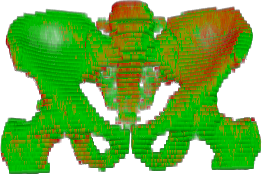
\includegraphics[width=\linewidth]{figures/research/cd03_0003_overlay_3d_gc}}
\vspace{1mm}
\end{minipage}
\hfill
\begin{minipage}[b]{0.48\linewidth}
  \centering
  \centerline{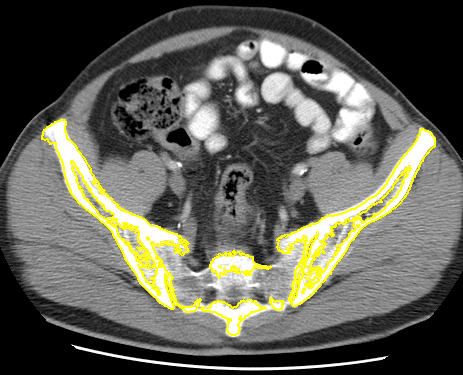
\includegraphics[width=\linewidth]{figures/research/d03_0003_Reg_Overlay_0015_cut}}
\vspace{1mm}
\end{minipage}\\
\begin{minipage}[b]{.48\linewidth}
  \centering
\centerline{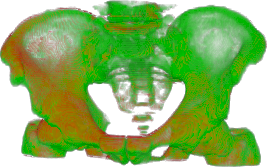
\includegraphics[width=\linewidth]{figures/research/sa_09_10_cut_3d_reg_overlay_gc}}
\vspace{1mm}
\end{minipage}
\hfill
\begin{minipage}[b]{0.48\linewidth}
  \centering
  \centerline{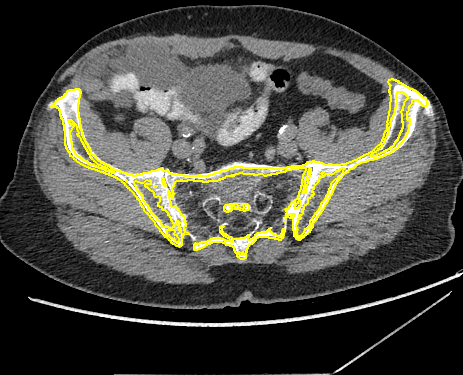
\includegraphics[width=\linewidth]{figures/research/SA_09_10_cut_Reg_Overlay_0056_cut}}
\vspace{1mm}
\end{minipage}
\caption{Registration of pelvic CT data: superimposed registered 3D bone
models (left column), and
bone contours of the registered template (yellow) overlaid on a CT slice of the observations (right column).
}
\label{fig:realct}
\end{figure}

%
% Christer
% Project Digital Geometry

\item 
\textbf{Digital Geometry}\\
Christer Kiselman\\
\ppartners{Shiva Samieinia, The Royal Institute of Technology; Adama Kon\' e, Universit\' e de Bamako I}
\ffunding{Stockholm University; The Royal Institute of Technology (KTH); International Science Programme; Universit\' e de Bamako I; Kingdom of Sweden}
\pperiod{1011-}
\aabstract{Digital planes i all dimensions are studied, which means that digital straightness is in focus.  However, straightness is conveniently understood as convexity together with concavity, which makes it natural to study also digital convexity, and therefore operations on digitally convex sets and functions.  Among the operations infimal convolution is of importance, including the operation of taking the marginal function.}

%
% Christer Project
% Euclid Straight Lines

\item 
\textbf{Euclid's Straight Lines}\\
Christer Kiselman\\
\ffunding{Kingdom of Sweden}
\pperiod{0701-}
\aabstract{The project is both linguistic and mathematical. We raise two 
questions on Euclid's Elements: How to explain that Propositions 16 and 27 in his first book do not follow, strictly speaking, from his postulates (or are perhaps meaningless)? and: What are the mathematical consequences of the meanings of the term eutheia, which we today often prefer to consider as different? 

The answer to the first question is that orientability is a tacit assumption.  The answer to the second is rather a discussion on efforts to avoid actual infinity, and having to (in some sense or another) construct equivalence classes of segments to achieve uniqueness. An article will appear in Normat, volume 62, formal year of publication 2014; actual year of publication 2015.}

%
% Christer
% Discrete Convolution Equations

\item 
\textbf{Discrete Convolution Equations}\\
Christer Kiselman\\
\ffunding{Kingdom of Sweden}
\pperiod{1201-}
\aabstract{We study solvability of convolution equations for functions with discrete support in $\mathbf{R}^n$, a special case being 
functions with support in the integer points.  The more general case is of interest for several grids in Euclidean space, like the 
body-centred and face-centered tesselations of three-space, as well 
as for the non-periodic grids that appear in the study of 
quasicrystals.  The theorem of existence of fundamental solutions by de Boor, H\"{o}llig \& Riemenschneider is generalized to general discrete supports, using only elementary methods.  We also study the asymptotic 
growth of sequences and arrays using the Fenchel transformation. Estimates using the Fourier transformation will be studied later.}

\clearpage

%----------------------------------------------------------------------------------------------------------------------------------------------
%----------------------------------------------------------------------------------------------------------------------------------------------
%----------------------------------------------------------------------------------------------------------------------------------------------

\subsection{Other projects}

% AAA

\item \textbf{Optical Character Recognition of Handwritten Texts}\\
Anders Brun, Ewert Bengtsson, Fredrik Wahlberg, Tomas Wilkinson, Kalyan Ram\\
\ppartners{Lasse M{\aa}rtensson, Dept.~of Scandinavian Languages, UU; Mats Dahll\"{o}f, Dept.~of Linguistics and Philology, UU}
\ffunding{Faculty of Languages and Humanities, UU and Vetenskapsr\r{a}det}
\pperiod{1008--}
\aabstract{Optical character recognition (OCR) is still, after nearly 100 years of research, an active area of research. Currently one of the frontiers is the recognition of handwritten text (HTR), in particular from historical documents. This year, we had a 2 month visit by guest researcher Alicia Forn\' es from Universitat Aut\` onoma de Barcelona. We submitted several grant applications and continued a collaboration with the Swedish Museum of Natural History. Promising results during the year include a novel visualization technique, image based word clouds (Fig. \ref{fig:OCR2}), large scale analysis of medieval letters, better techniques for document binarization and cluster analysis of letter shapes (Fig. \ref{fig:OCR1}).}

\begin{figure}[!htbp]
\centering
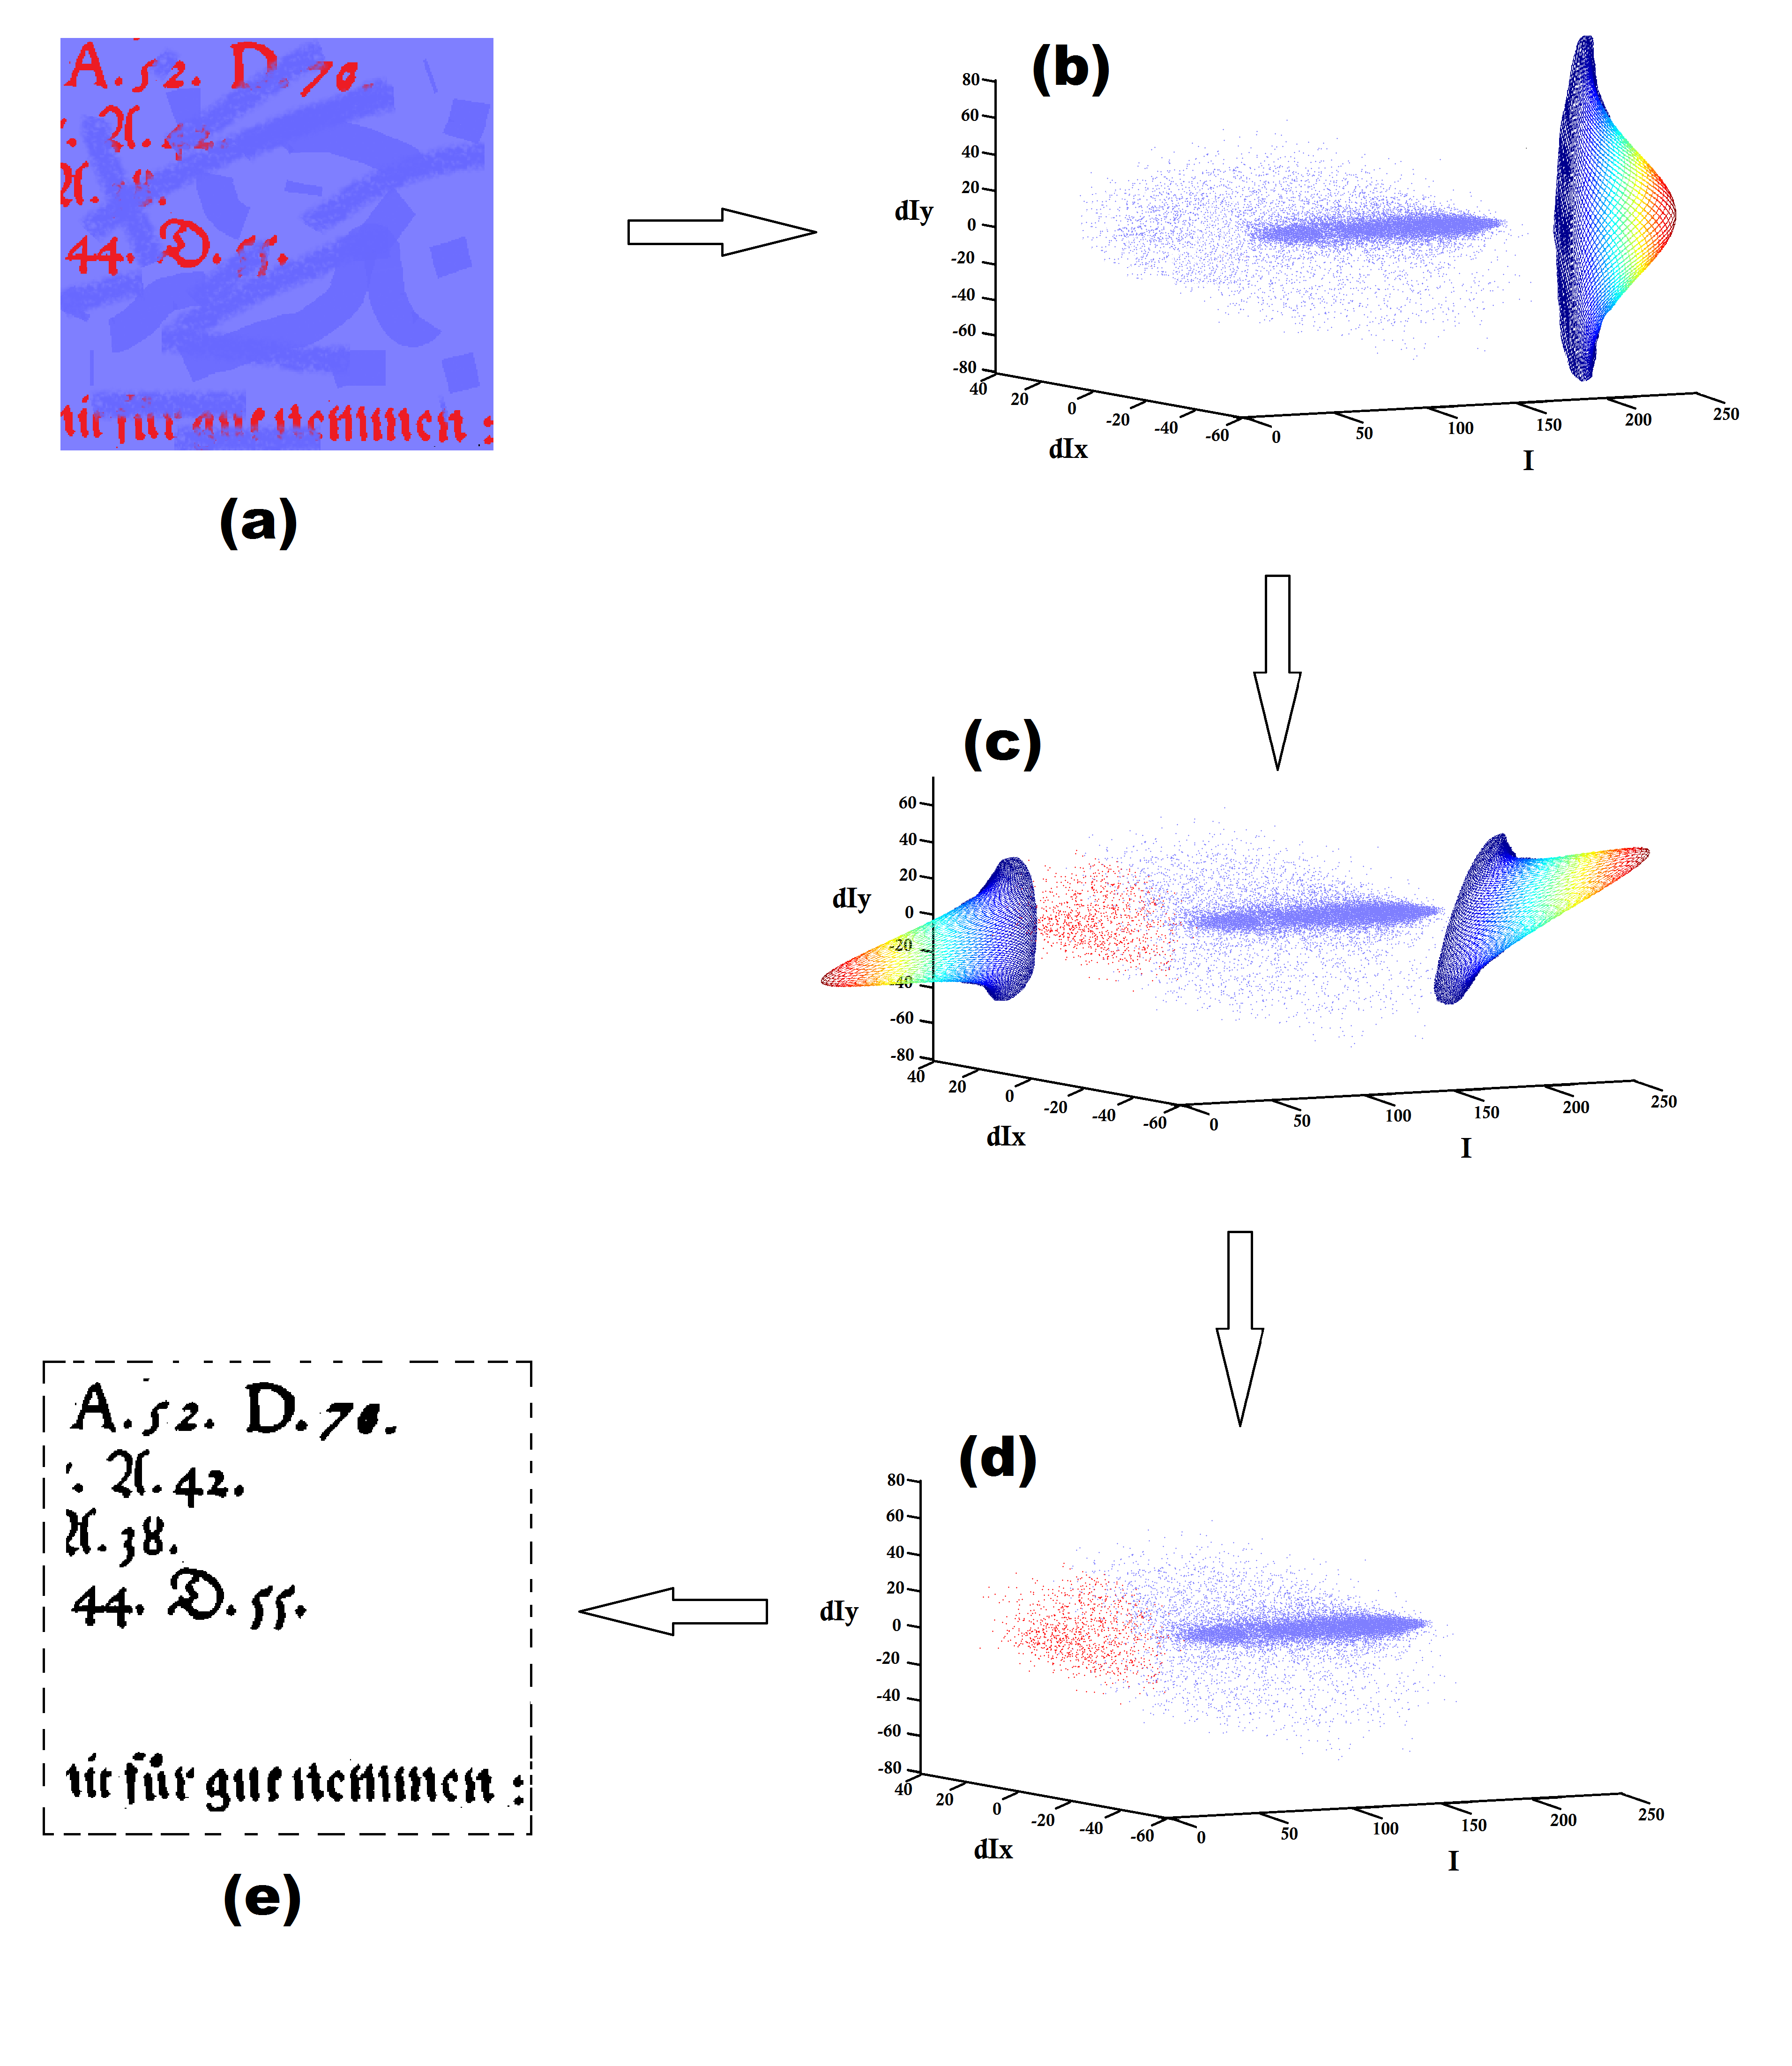
\includegraphics[width=0.8\textwidth]{figures/research/BgFgClus.png}
\caption{\label{fig:OCR1} Hierarchical Mean Shift clustering based binarization procedure is outlined here with input as shown in (a) and output as indicated in (e) through separation of foreground and background clusters in a three dimentional space of intensity, x-derivative, y-derivative at each pixel as shown in (b)-(d).} 
\end{figure}

\begin{figure}[!htbp]
\centering
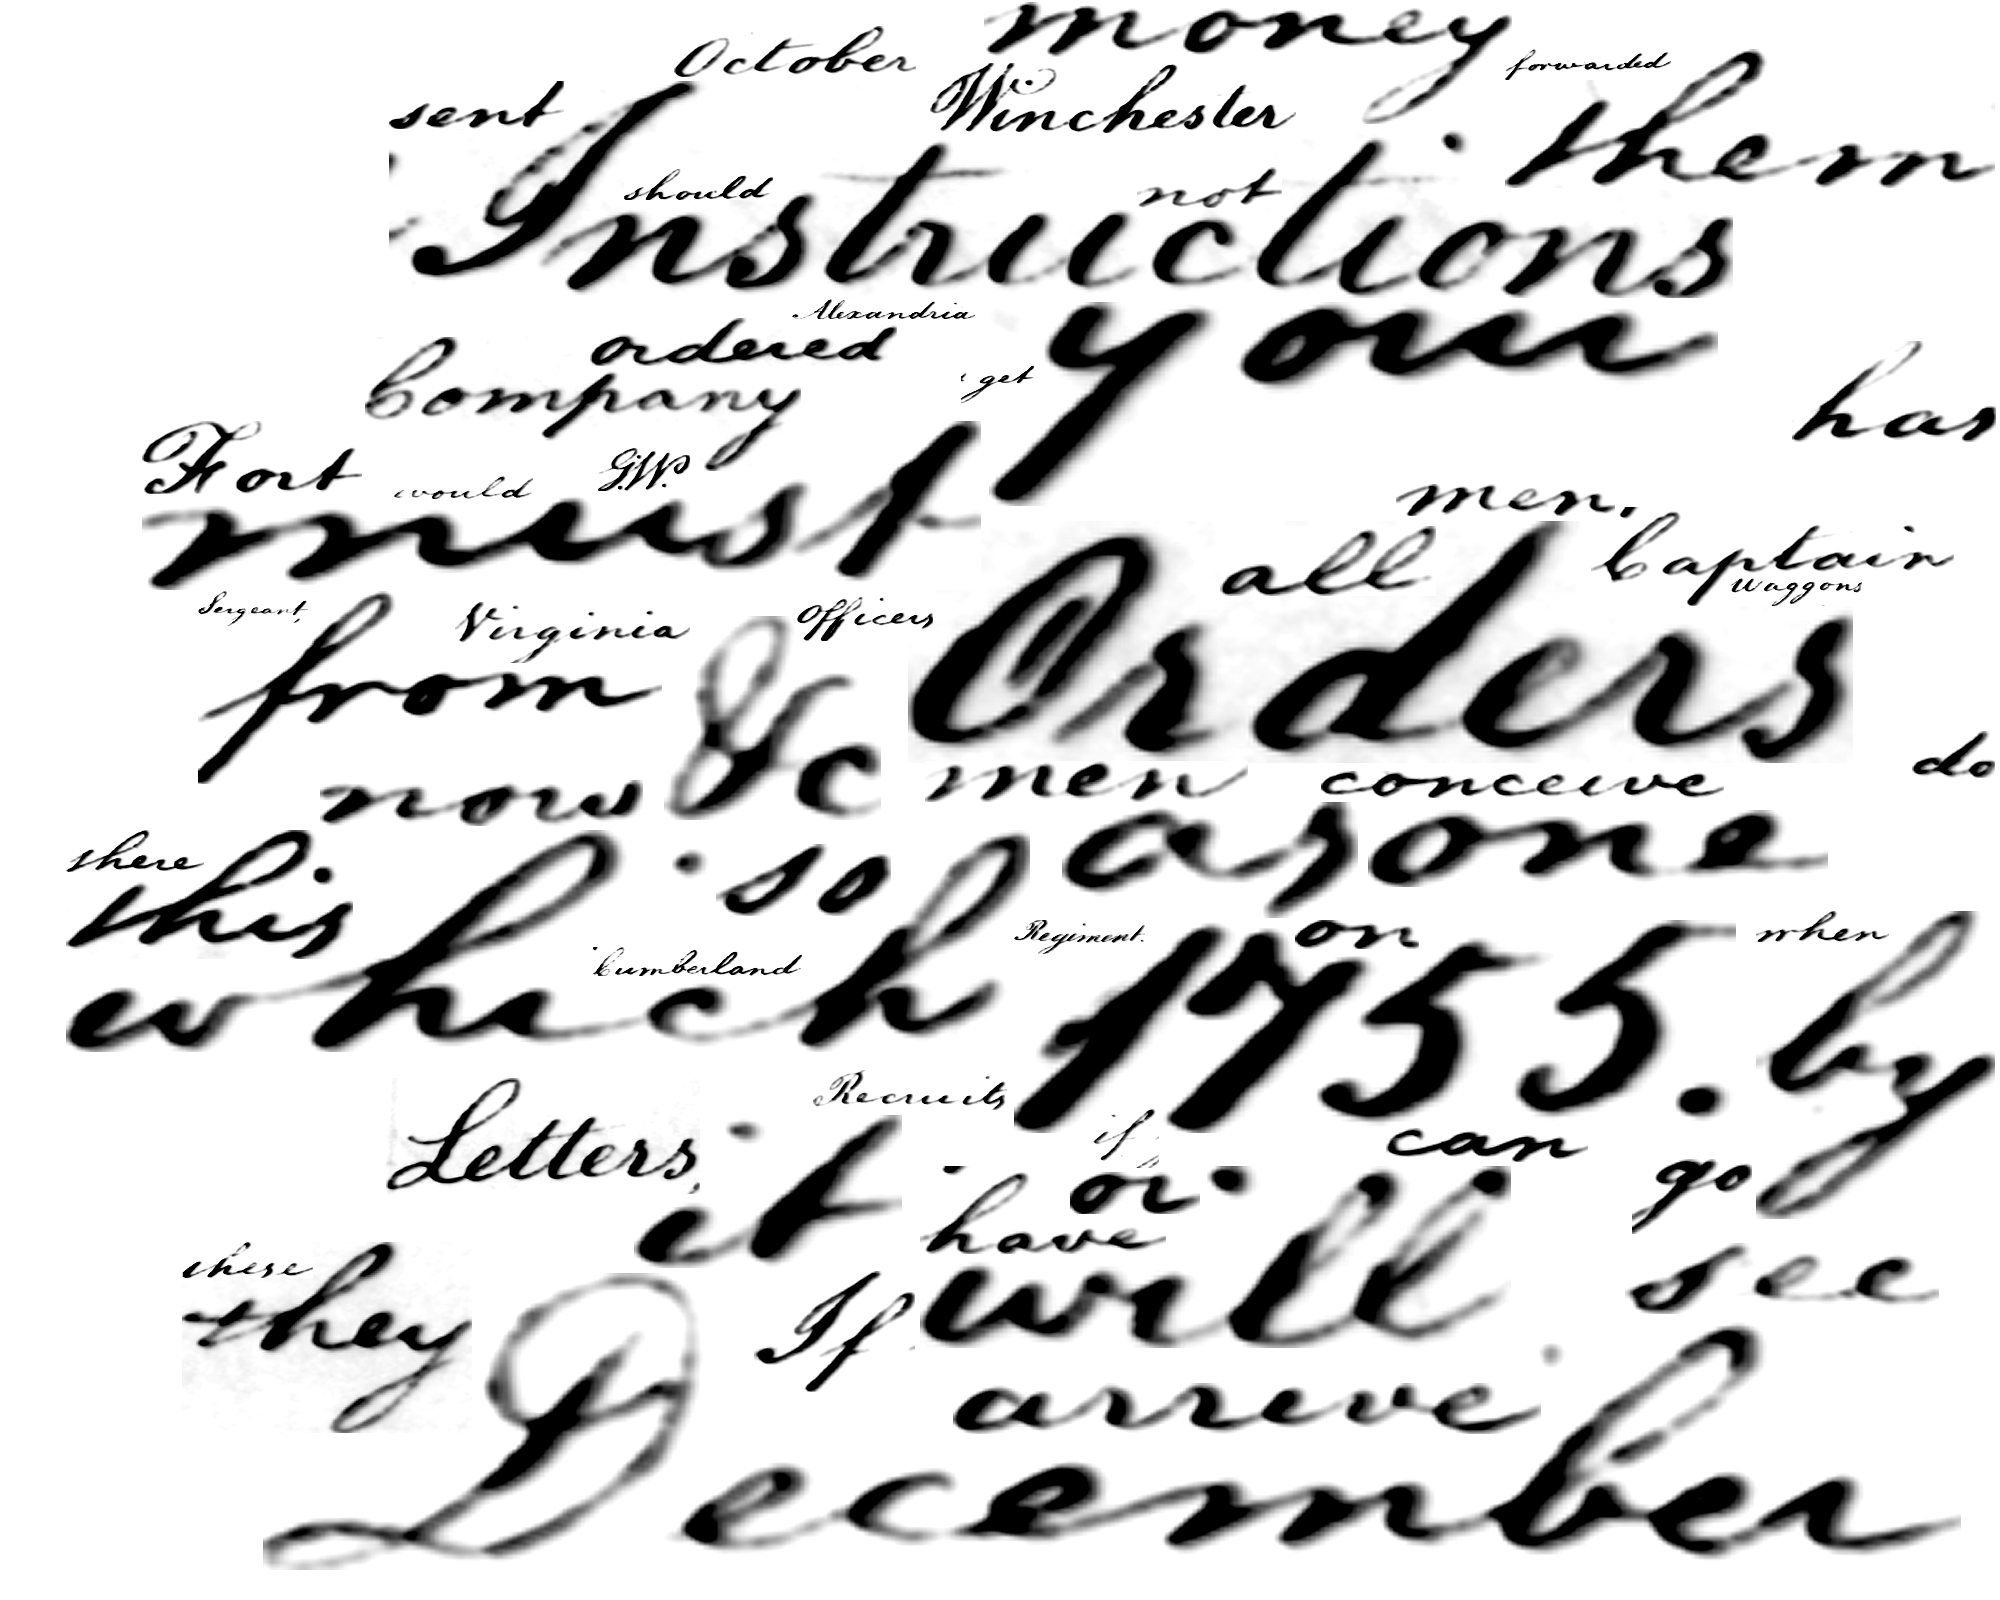
\includegraphics[width=0.8\textwidth]{figures/research/word_cloud_washington.png}
\caption{\label{fig:OCR2} An image-based word cloud generated from a scanned collection of a 18th century letters written by George Washington. The cloud approximately contains the most frequently occuring images of words in the collection.} 
\end{figure}

%BBB

\item
\label{proj:geomemories}
\textbf{GeoMemories}\\
Anders Hast\\
\ppartners{Andrea Marchetti, Salvatore Minutoli, Alessandro Prosperi, Alessandro Lugari, Maurizio Tesconi, Beatrice Rapisarda, Matteo Abrate, Clara Bacciu, Davide Gazz\'e, Sergio Bianchi, Istituto di Informatica e Telematica (IIT), Pisa, Italy}
\aabstract{The GeoMemories project is aimed at making publicly available, through web access, heritage preserved in the archives of Aerofototeca Nazionale in Rome, which contains photographs covering the Italian territory from the end of 1800 till modern days. The web application is based on google earth but oriented towards the management of the temporal variable, so that geospatial changes can be monitored over time. The historical aerial photos need to be digitized, illumination corrected, orthorectified, georeferenced and finally stitched together. Anders Hast spent one year (2011) at IIT, CNR in Pisa Italy as an ERCIM fellow working with image processing and computer vision aspects in the project. Since returning to UU he is a research associate at IIT, CNR and continues working with the project and focus has been on how to improve the algorithms needed and several papers have been published. Recently the challenges and advantages of stereo visualisation of the historical archive has been investigated.}

%\begin{figure}[!htbp]
%\centering
%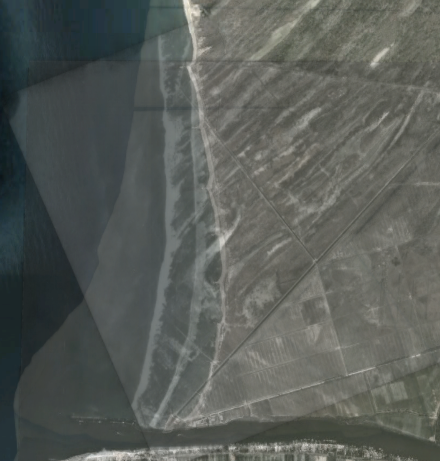
\includegraphics[width=0.6\textwidth]{figures/research/foce_all.png}
%\caption{\label{fig:pisa} This blended photo makes it possible to study how the costal shore line outside Pisa has changed and moved in time and space. Images from four different sources are blended together in the GeoMemories application to show the environmental changes. The images are a cadastral map that was published 1765, officially issued by Pietro Leopoldo the Grand Duke of Tuscany, a RAF photo from 1943, an aerial photo from 1962 and a recent Google Earth photo.} 
%\end{figure}

%CCC

\item \textbf{Image Analysis for Landscape Analysis}\\
Anders Brun\\
\ppartners{Bo Malmberg, Michael Nielsen, Dept.~of Human Geography, Stockholm University; Anders W\"{a}stfelt, Dept.~of Economics, SLU}
\ffunding{UU/SU}
\pperiod{0901--}
\aabstract{This project is a collaboration with researchers at SU and SLU. It aims to derive information about the landscape (rural and city) from satellite images. The project focuses on using texture analysis of images, rather than only pixelwise spectral analysis, to segment the image into different meaningful regions. One journal manuscript was accepted during 2013 and the collaboration with the GLEAN project at the department of Political Science at Stockholm University has continued.}

%DDD

%\item \textbf{Dual-domain Visual Exploration of Urban Solar Potential}\\
%Stefan Seipel\\
%\ppartners{Joakim Wid\'{e}n, David Lingfors, Solid State Physics, Dept.~of Engineering Sciences, UU}
%\ffunding{University of G\"{a}vle; TN-faculty, UU}
%\pperiod{1211--}%20150801}
%\aabstract{This project aims to improve the planning and design of solar electricity installations in the urban environment. One major objective of these studies is to enable a highly detailed temporal and spatial analysis of the expected solar yield, which becomes increasingly important for optimal load balance in electric power networks. In our research we develop a 3D simulation model that integrates geographical data and detailed 3D urban models with temporal solar irradiance and climate data. According to our model the predicted solar yield becomes a multi-dimensional function of several design-specific parameters that are interactively explored by a human expert.  This project is an interdisciplinary initiative that involves researchers from Energy Systems and from Computer Science at UU and the University of G\"{a}vle. During the first year, a demonstrator system for the interactive exploration of the design parameter space has been developed. Our method and the demonstrator system have been published in two international conferences in 2013. Forthcoming research in this project will concern the refinement and validation of computational models, as well new methods for interactive visual exploration.}

% FFF

\item 
\label{proj:honey_bees}
\textbf{Tracking Honey Bees and Their Interactions}\\
Cris Luengo\\
\ppartners{Olle Terenius, Ingemar Fries, Joachim Rodrigues de Miranda, Eva Forsgren, Barbara Locke, Dept.~of Ecology, SLU; Fredrik Liljeros, Dept.~of Sociology, Stockholm University}
\ffunding{{\AA}ke Wiberg foundation; and S-faculty, SLU}
\period{1003--}\\
\aabstract{In this project, we are creating a system in which we can observe a portion of a bee hive (containing about one thousand individuals, each tagged with a unique identifier on its back) over days or weeks. Bees will be free to enter and exit the hive, and the environment will be set up to be as natural as possible for the bees. The purpose is to observe the natural behaviour of the bees, and record the type and duration of interaction between individuals. During 2014, we applied for funding to continue this work.}
%\begin{figure}[htpb!]
%\centering
%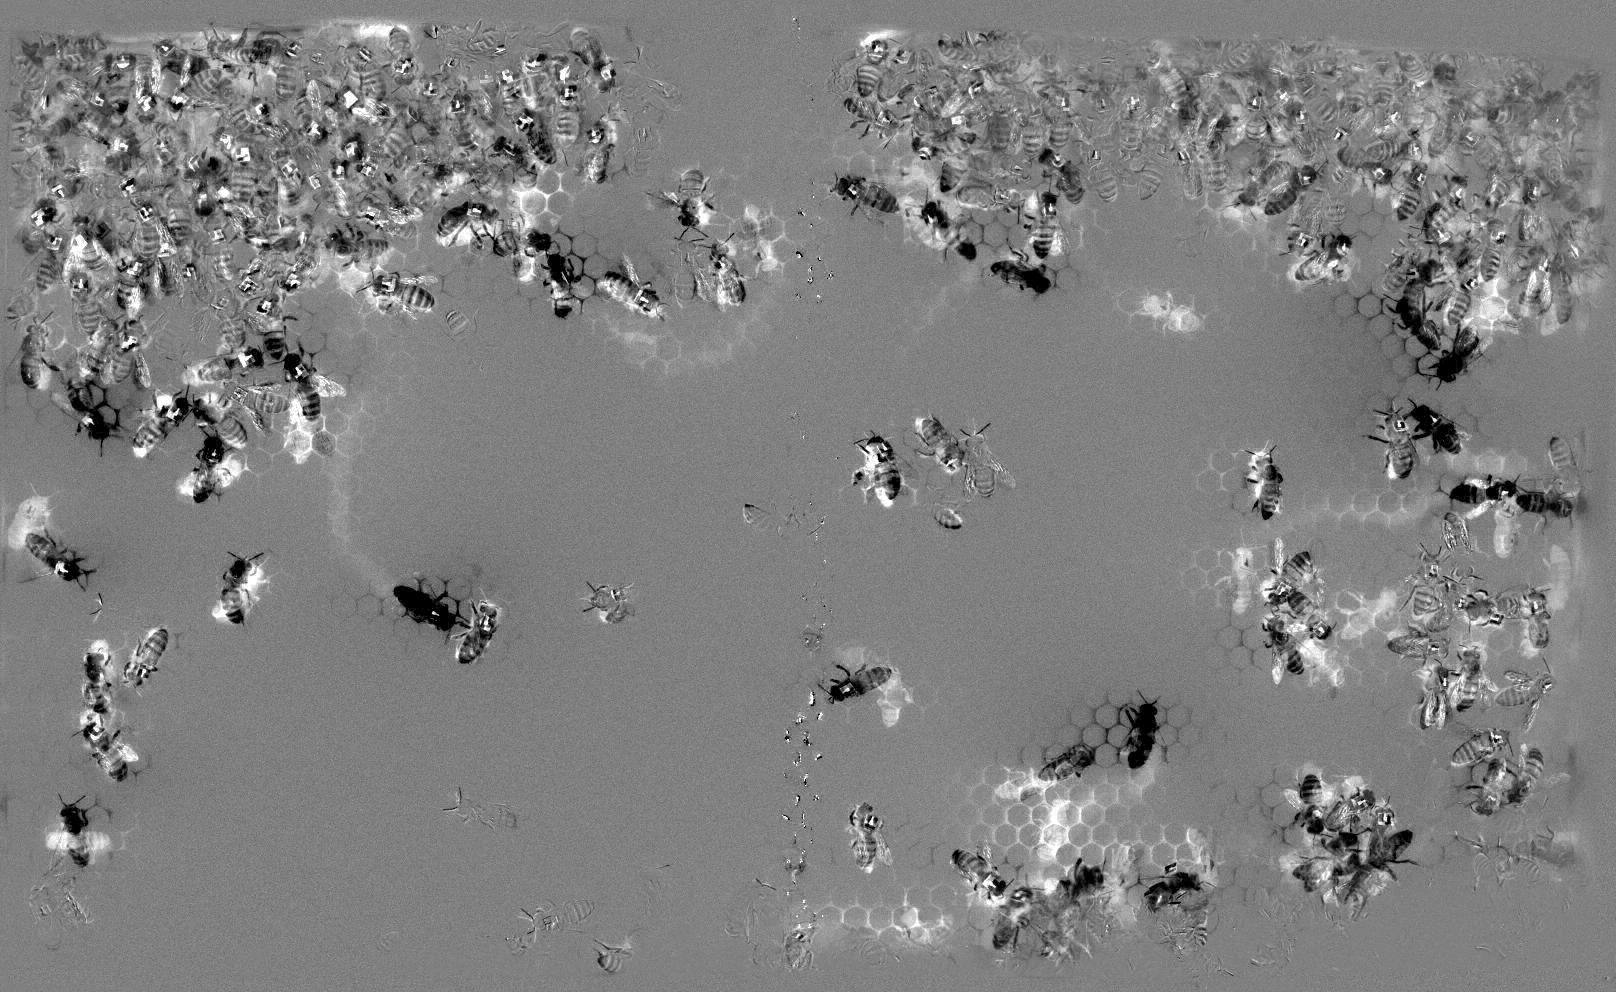
\includegraphics[width=0.85\textwidth]{figures/research/bees1.png}
%\caption{\label{fig:bees} The result of a method for background subtraction, where only moving individuals are still visible.} 
%\end{figure}

%HHH

\item
\label{proj:dipimage}
\textbf{DIPimage and DIPlib}\\
Cris Luengo\\
\ppartners{Bernd Rieger, Lucas van Vliet, Quantitative Imaging Group, Delft University of Technology, The Netherlands; Michael van Ginkel, Unilever Research and Development, Colworth House, Bedford, UK}
\ffunding{S-faculty, SLU}
\pperiod{0807--}
\aabstract{DIPimage is a MATLAB toolbox for scientific image analysis, useful for both teaching and research (\url{http://www.diplib.org}). It has been in active development since 1999, when it was created at Delft University of Technology. In 2008, when Cris Luengo moved to Uppsala, CBA was added to the project as a main development site. DIPlib, created in 1995, is a C library containing many hundreds of image analysis routines. DIPlib is the core of the DIPimage toolbox, and both projects are developed in parallel. Because DIPlib provides efficient algorithms, MATLAB is useful for image analysis beyond the prototyping stage. Together, MATLAB and DIPimage form a powerful tool for working with scalar and vector images in any number of dimensions.

Versions 2.6 and 2.7 were released in 2014. Version 2.6 added the option to do arithmetic operations without changing the data type of the image, useful when working with very large images. We also fixed a major bug that appeared due to some undocumented internal change in MATLAB, which caused the output images of certain functions to be copied unnecessarily. Version 2.7 added the  possibility to record macros (as MATLAB M-files), added a few new functions, and fixed many bugs. In particular, we had to make many changes for compatibility with MATLAB's new graphic system.} 

% UPPMAX

\item 
\textbf{UPPMAX Cluster Computing}\\
Petter Ranefall, Ida-Maria Sintorn, Carolina W\"{a}hlby\\
\ppartners{Hans Karlsson, Elias Rudberg, Ola Spjuth, UPPMAX}
\ffunding{SciLife Lab Uppsala; eSSENCE; Dept.~of IT, UU}
\pperiod{1110-}
\aabstract{Life science applications generate a huge amount of image data that has to be stored and analysed in an efficient way. This project
is focused on providing easy access to high-performance computers and large-scale storage. In collaboration with Uppsala Multidisciplinary Center for Advanced Computational Science (UPPMAX) image analysis software are being installed and maintained on the cluster. Database solutions with easy web access to image data are also being developed and maintained. This project has also provided workshops and seminars to help life science researchers to get started and use the resources. Several new large-scale image analysis projects using the computer cluster were initiated in 2014.}

\clearpage

\end{enumerate}

\end{document}

